\section{Results in \llll channel}
\label{sec:hmhzz_result_4l}

The statistical treatment in searching for heavy resonances in $ZZ \rightarrow \llll$ final state is described in this section.
Results are presented in both cut- and MVA- based analysis.

\subsection{Statistical procedure}

The upper limits on heavy resonances are obtained using the unbinned profile likelihood fits.
\mfl is the discriminant.
The likelihood function is a product of a Poisson term representing the probability of observing $n$ events 
and a weighted sum of both signal and background probability distribution functions (PDFs) evaluated at all observed events.
\begingroup
\small
\begin{equation}
  {\cal L } (x_{1}..x_{n}| \sigma_{ggF}, \sigma_{VBF}) = \textrm{Pois}(n|S_{ggF} + S_{VBF} + B)  \left[ \prod\limits^{n}_{i=1}
  \frac{S_{ggF} f_{\textrm{ggF}}(x_{i}) + S_{VBF} f_{\textrm{VBF}}(x_{i}) + B f_{\textrm{B}}(x_{i})}{S_{ggF} + S_{VBF} + B}
  \right]
\end{equation}
\endgroup
where $f_X$s are the probability distribution functions of signal and backgrounds modelled in section~\ref{sec:signal_model} and ~\ref{sec:hmhzz_bkg}, 
$S_X$ and $B$ are the normalizations of signal and sum of backgrounds.

The parameters of interest (POI) in the search is $\sigma_{ggF}$ (and $\sigma_{VBF}$ only for NWA signal), which is the cross section of signal model in ggF (and VBF) production mode.
In the case of there are two POIs, when testing one POI, the other one is profiled along with other nuisance parameters (except left unconstrained) during the minimization. 
These POIs enter the likelihood inside the expected signal yields $S_{ggF}$ and $S_{VBF}$ as:
\begingroup
\small
\begin{equation}
S_{ggF(VBF)} = \sigma_{ggF(VBF)} \times BR(S\rightarrow ZZ) \times A \times C \times \int\mathcal{L}
\end{equation}
\endgroup
where $A\times C$ is the signal acceptance as parameterized in~\ref{sec:hmhzz_signal_acc}, and $\int\mathcal{L} = \lumi $ is the integrated luminosity of the dataset.

The dependence of the expected number of signal and background events (normalizations) and the shape of the PDFs on the systematic uncertainties measured in section~\ref{sec:hmhzz_sys} 
is described by a set of nuisance parameters (NPs) $\theta_{i}$.
The Gaussian constraints are applied to those NPs.
The constraints are implemented as additional `penalty' terms added to the likelihood which increase the negative log-likelihood when any nuisance parameter is shifted from its nominal value. 
The final likelihood function ${\cal L } ( \sigma_{ggF}, \sigma_{VBF},\mH,\theta_{i})$ is therefore a function of  $\sigma_{ggF}, \sigma_{VBF} , \mH$, and $\theta_{i}$.

Furthermore, the normalization of SM background $pp\to ZZ$, including both \qqZZ\ and \ggZZ, is a free parameter ($\mu_{ZZ}$) and profiled during the minimization.
Floating $ZZ$ normalization in fit takes the advantage of reducing the dependence on theory predictions and their associated uncertainties,
especially given that the increased data luminosity would provide precise determination of the SM $ZZ$ background rate.

At the end, the upper limit on production cross-section $\sigma_{ggF(VBF)}$ at a given heavy resonance model is obtained by setting the mass of signal $m_{H}$ parameter as constant at the desired value,
and maximising the likelihood function with respect to nuisance parameters.
%The test statistics $q_\mu$ is used to set upper limits following \cite{CowanTestStatistics}. 
The $CL_{\textrm{s}}$ \cite{cls} method is used to obtain exclusion limits.
%In order to measure the compatibility of the data with the background-only hypothesis ($\sigma_{ggF}=\sigma_{VBF}=0$), the test statistic $q_{0}$ is used.

\subsection{Likelihood fit under background-only hypothesis for MVA-based analysis}

Both MVA- and cut-based analysis are studied by performing likelihood fit to the (pseudo-) data under the background-only hypothesis and under different signal models.
Due to the same background estimation and modelling procedures, as well as the same method of systematic measurements,
this section only shows the results of background-only fits for MVA-based analysis under the model of heavy Higgs resonance with narrow-width as an example.
The final results of interpretation in both MVA- and cut- based analysis in all signal models described in section~\ref{sec:signal_model} will be measured in next section.

First of all, table~\ref{tab:postfit_4lyields} summarized the expected and observed number of events for region of $\mfl > 200~\gev~$ together with their systematic uncertainties after background-only fit.
The post-fit \mfl spectrum in each category is shown in figure~\ref{fig:m4l_postfit}.

\begin{table}[tbp]
    \caption{\label{tab:postfit_4lyields}
      Expected and observed numbers of events for $\mfl > 200~\gev{}$, 
      together with their systematic uncertainties, 
      for three MVA-based categories.
      The expected number of events, as well as their uncertainties, are obtained
      from a likelihood fit to the data under the background-only hypothesis.
      The uncertainties of the $ZZ$ normalisation factors, presented in table~\ref{tab:muZZ_bonly_dnn},
      are also taken into account.
    }
    \centering

    \footnotesize
    \resizebox{\textwidth}{!}{
      \begin{tabular}{l r@{ $\pm$ }l r@{ $\pm$ }l r@{ $\pm$ }l r@{ $\pm$ }l r@{ $\pm$ }l }
        \toprule
        \multirow{2}{*}{Process} & \multicolumn{2}{c}{VBF-enriched category} & \multicolumn{6}{c}{ggF-enriched categories}  & \multicolumn{2}{c}{the ``rest'' category} \\
        & \multicolumn{2}{c}{} & \multicolumn{2}{c}{$4\mu$ channel} & \multicolumn{2}{c}{$2e2\mu$ channel} & \multicolumn{2}{c}{$4e$ channel}  & \multicolumn{2}{c}{} \\ 
        \midrule
  
        \qqZZ	&	11	&	4	&	232	&	10	&	389	&	17	&	154	&	7	&	2008	&	47	\\
        \ggZZ	&	3	&	2	&	37	&	6	&	64	&	10	&	26	&	4	&	247	&	19	\\
        \ZZ (EW)	&	4.1	&	0.4	&	4.5	&	0.2	&	7.5	&	0.4	&	3	&	0.2	&	14.3	&	0.7	\\
        \Zjet,\ttbar	&	0.08	&	0.02	&	0.6	&	0.1	&	1.7	&	0.4	&	0.8	&	0.1	&	8.8	&	2.1	\\
        \ttv,\vvv	&	0.97	&	0.1	&	9.8	&	0.2	&	17.5	&	0.4	&	7.8	&	0.2	&	21.9	&	0.5	\\
        \midrule
        Total background	&	19	&	4.5	&	285	&	11.7	&	479	&	19.7	&	192	&	8.1	&	2301	&	50.7	\\
        
        \midrule
        Observed  & \multicolumn{2}{c}{19} & \multicolumn{2}{c}{271} & \multicolumn{2}{c}{493} & \multicolumn{2}{c}{191} & \multicolumn{2}{c}{2301} \\
        \bottomrule
      \end{tabular}
    }
\end{table}

\begin{figure}[!ht]
  \begin{center}
  \subfloat[]{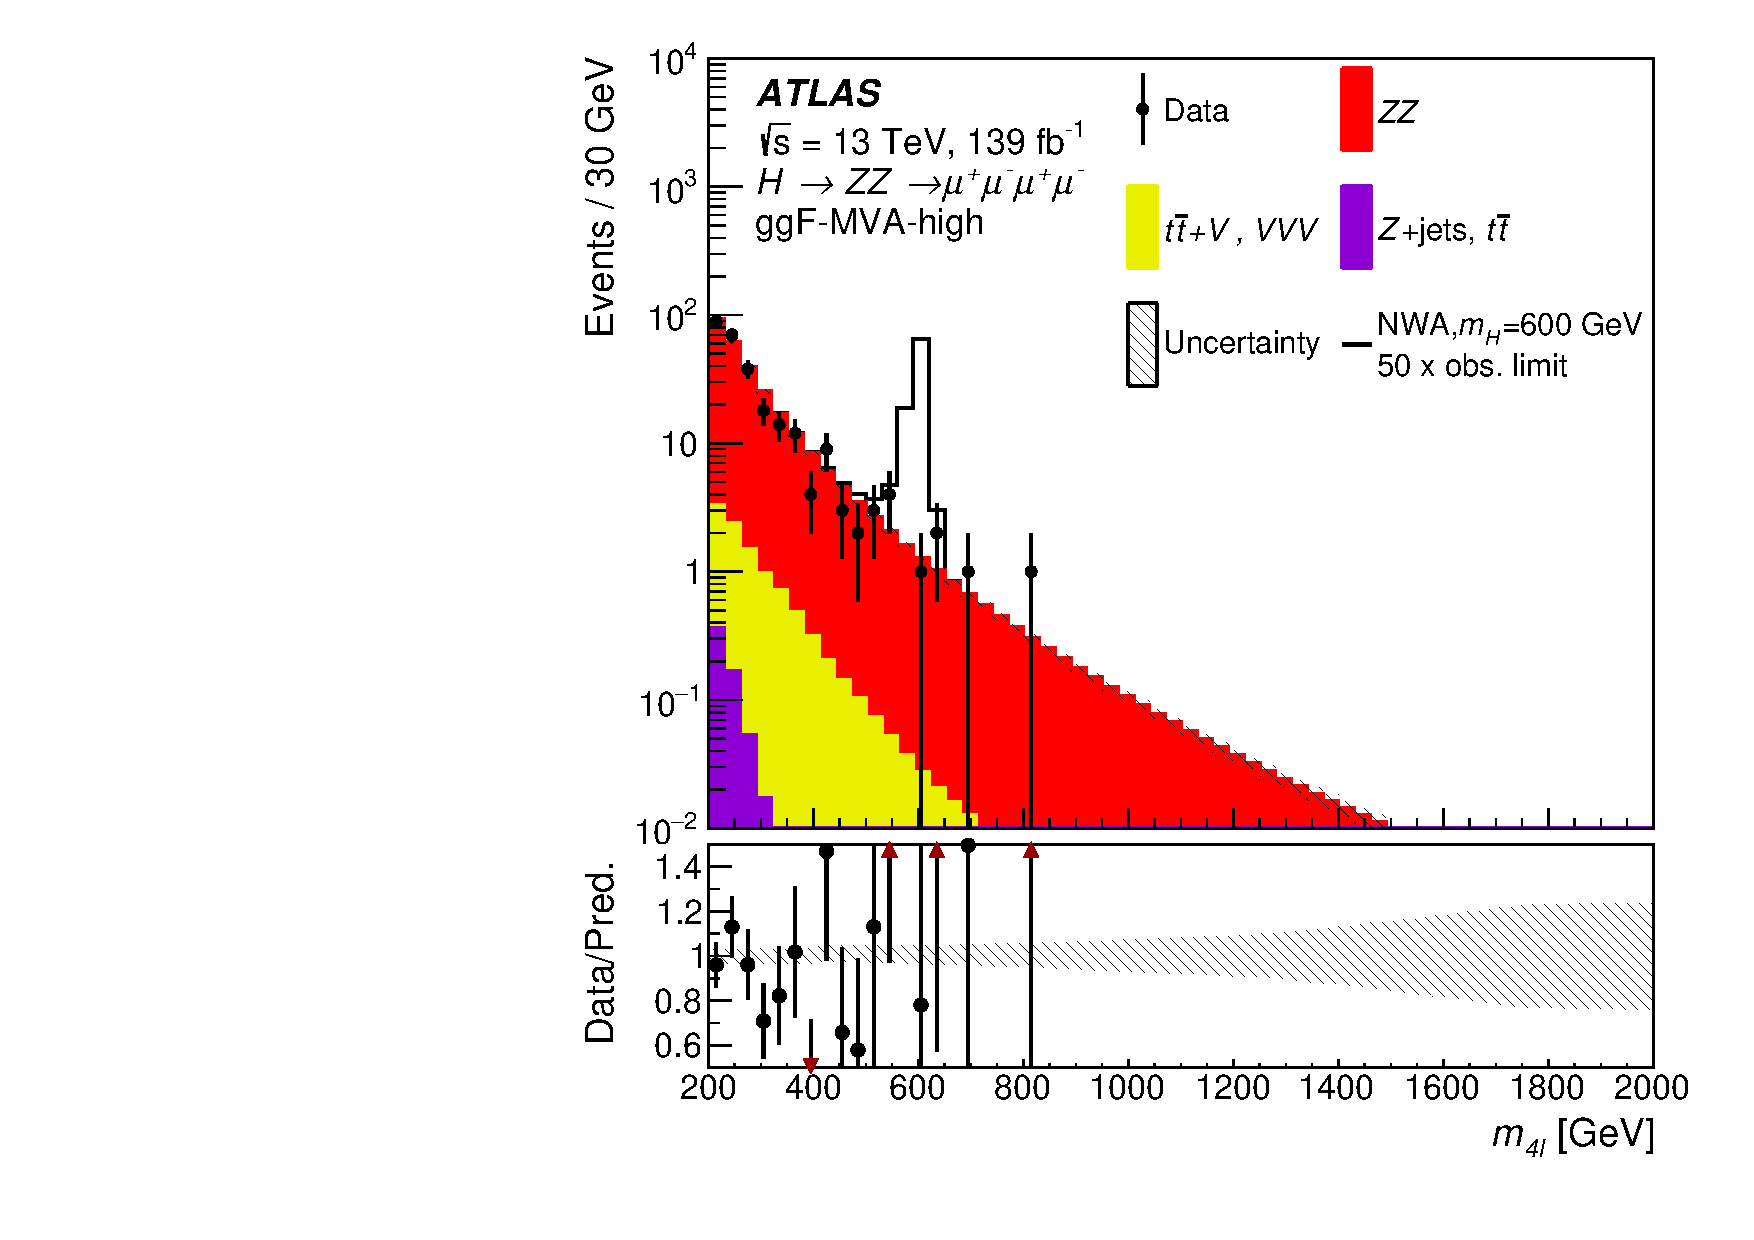
\includegraphics[width=0.32\textwidth]{figures/HMHZZ/results/4l_postfit_m4l_ggF_4mu.pdf}} 
  \subfloat[]{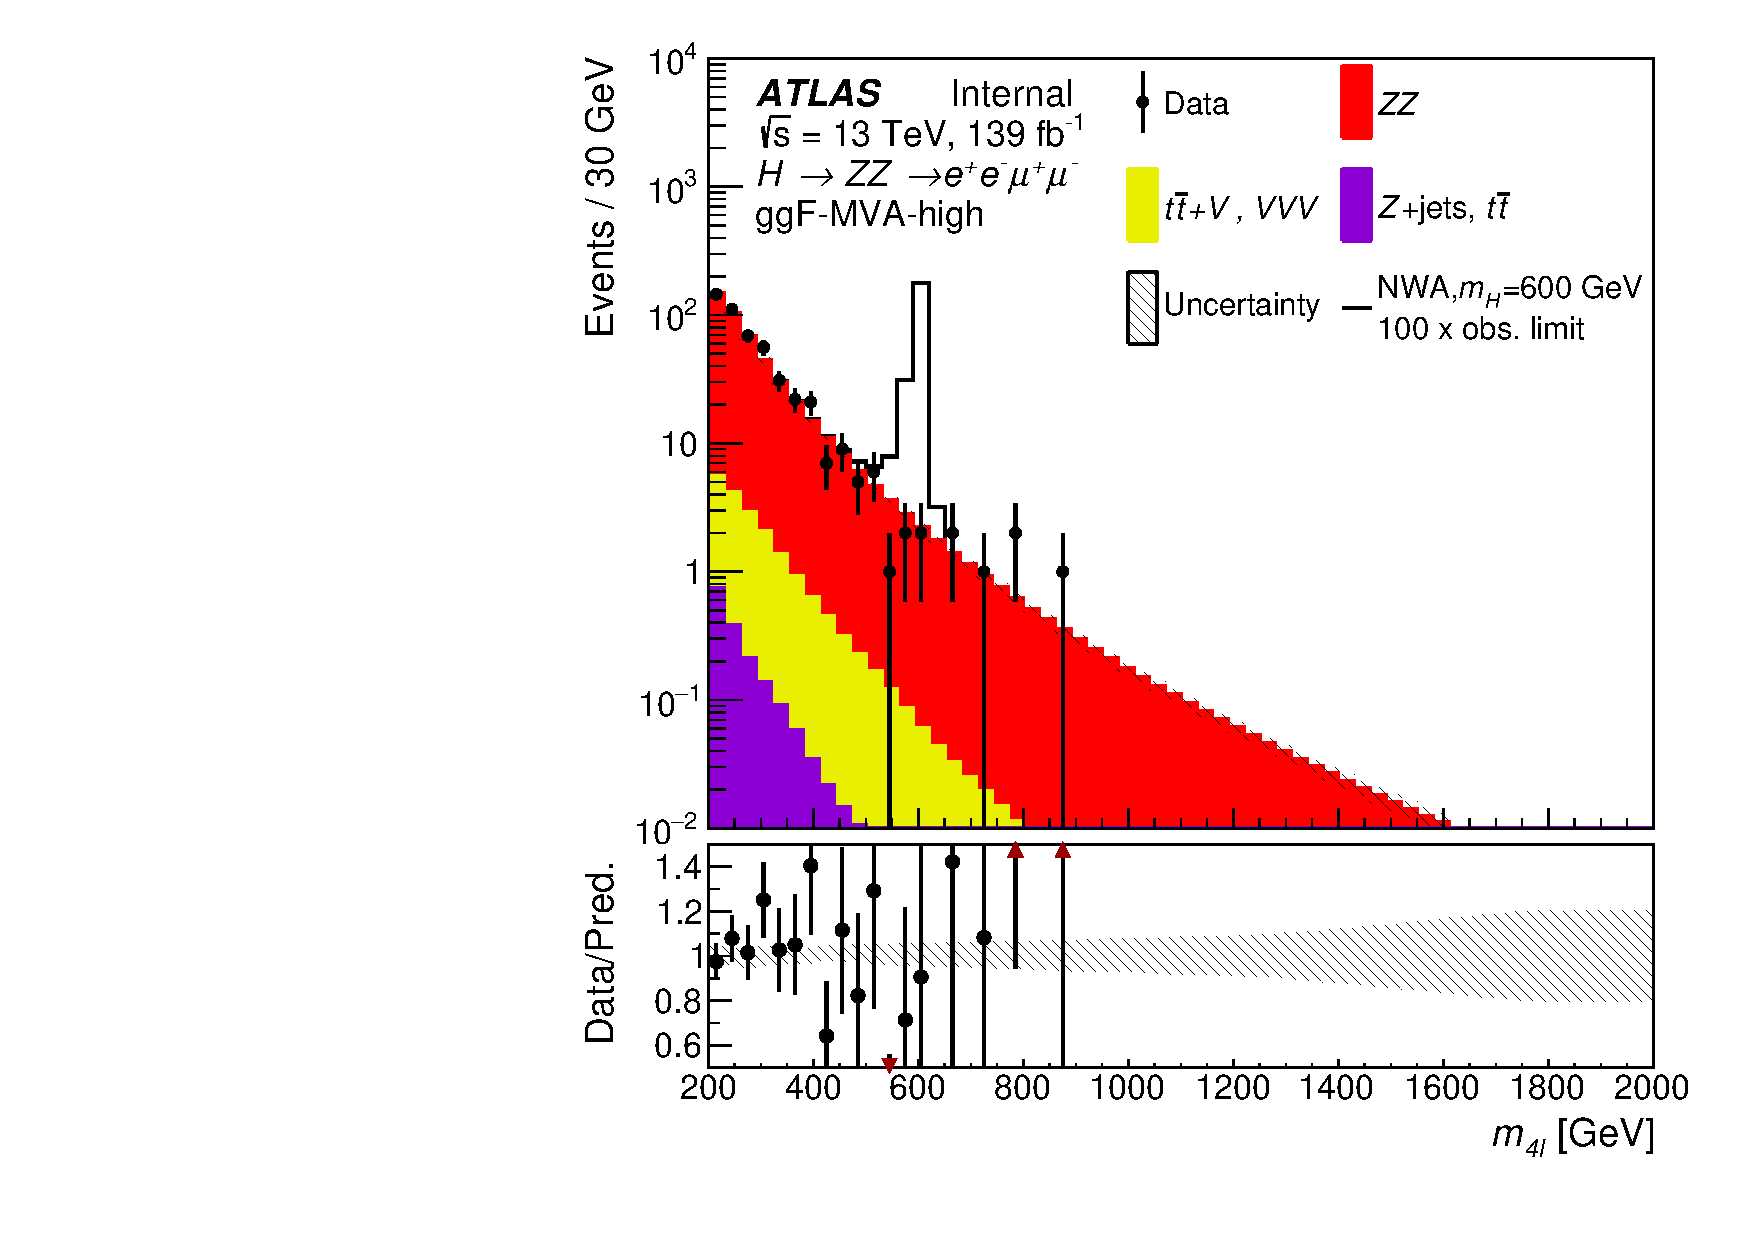
\includegraphics[width=0.32\textwidth]{figures/HMHZZ/results/4l_postfit_m4l_ggF_2mu2e.pdf}}
  \subfloat[]{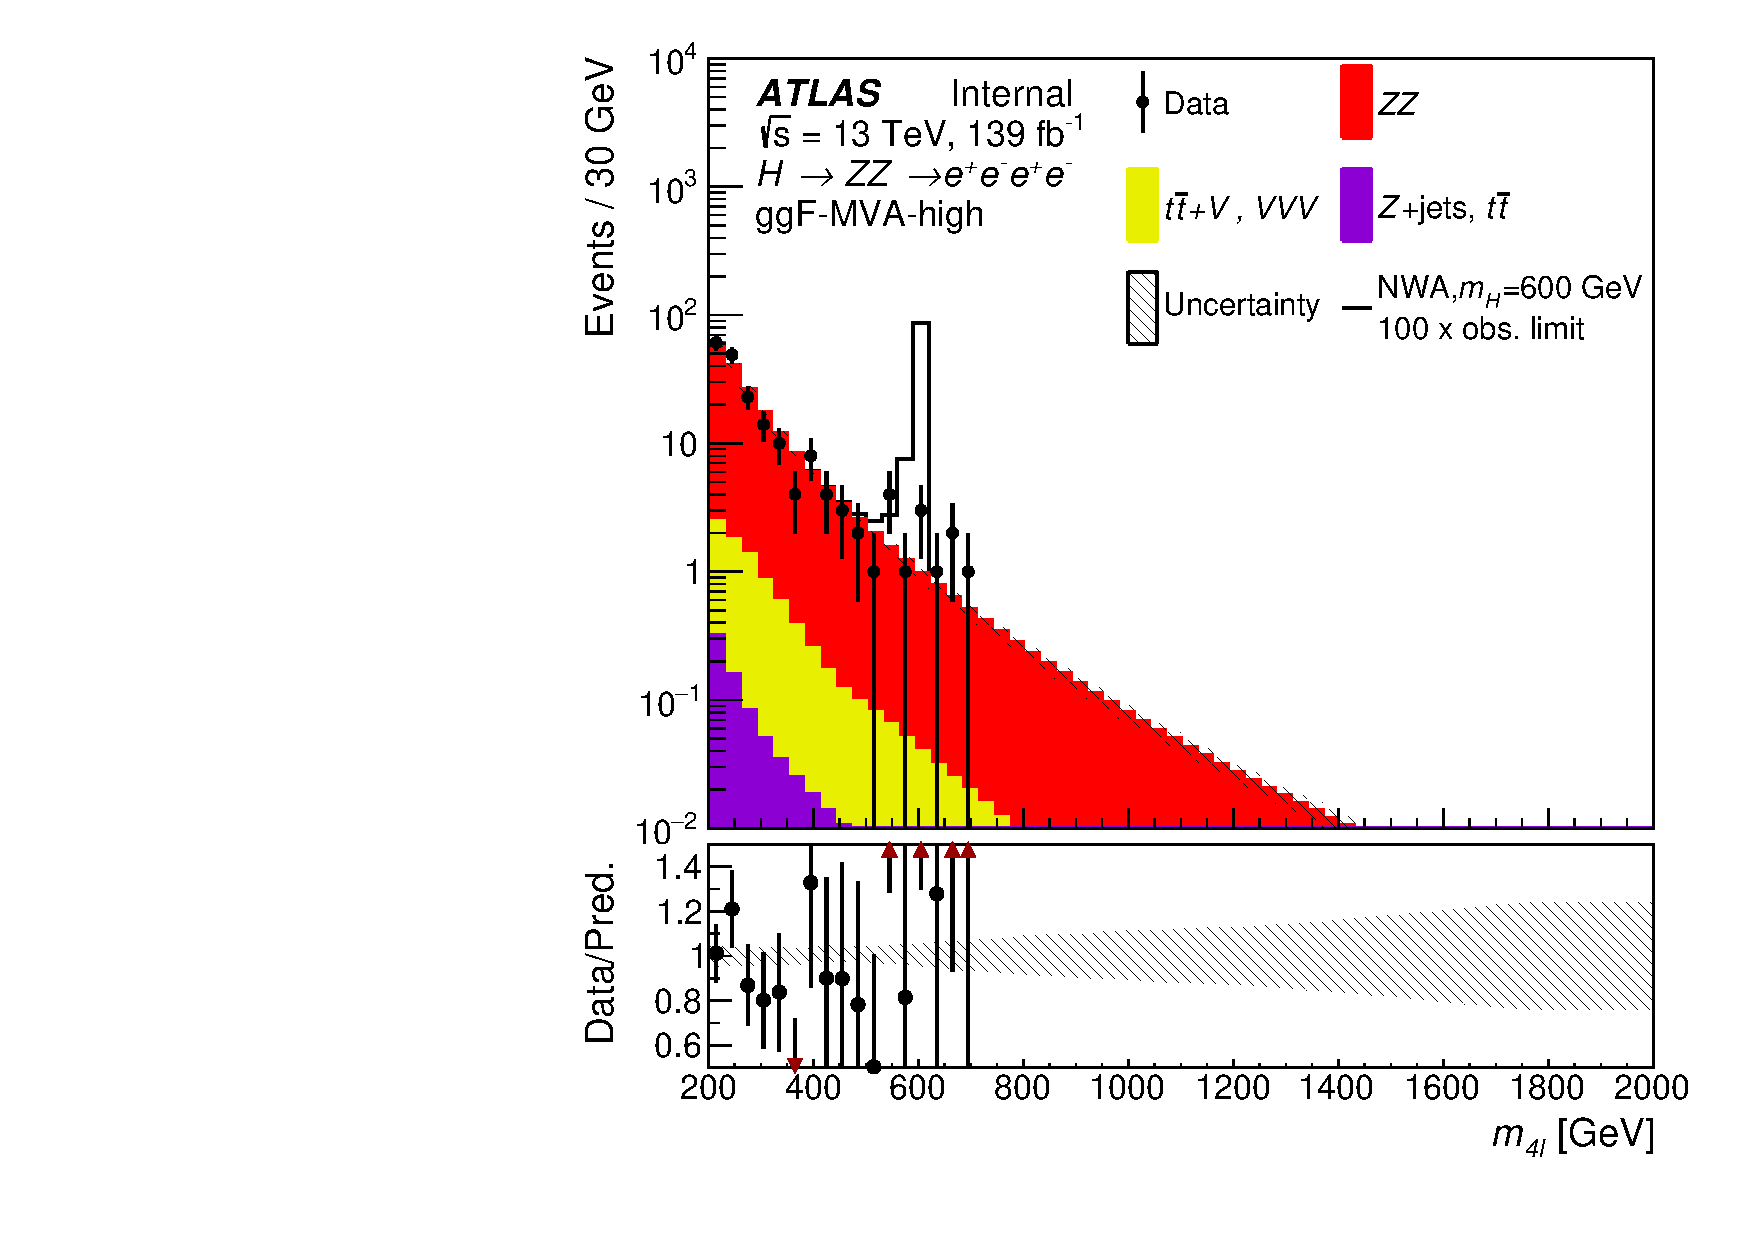
\includegraphics[width=0.32\textwidth]{figures/HMHZZ/results/4l_postfit_m4l_ggF_4e.pdf}} \\
  \subfloat[]{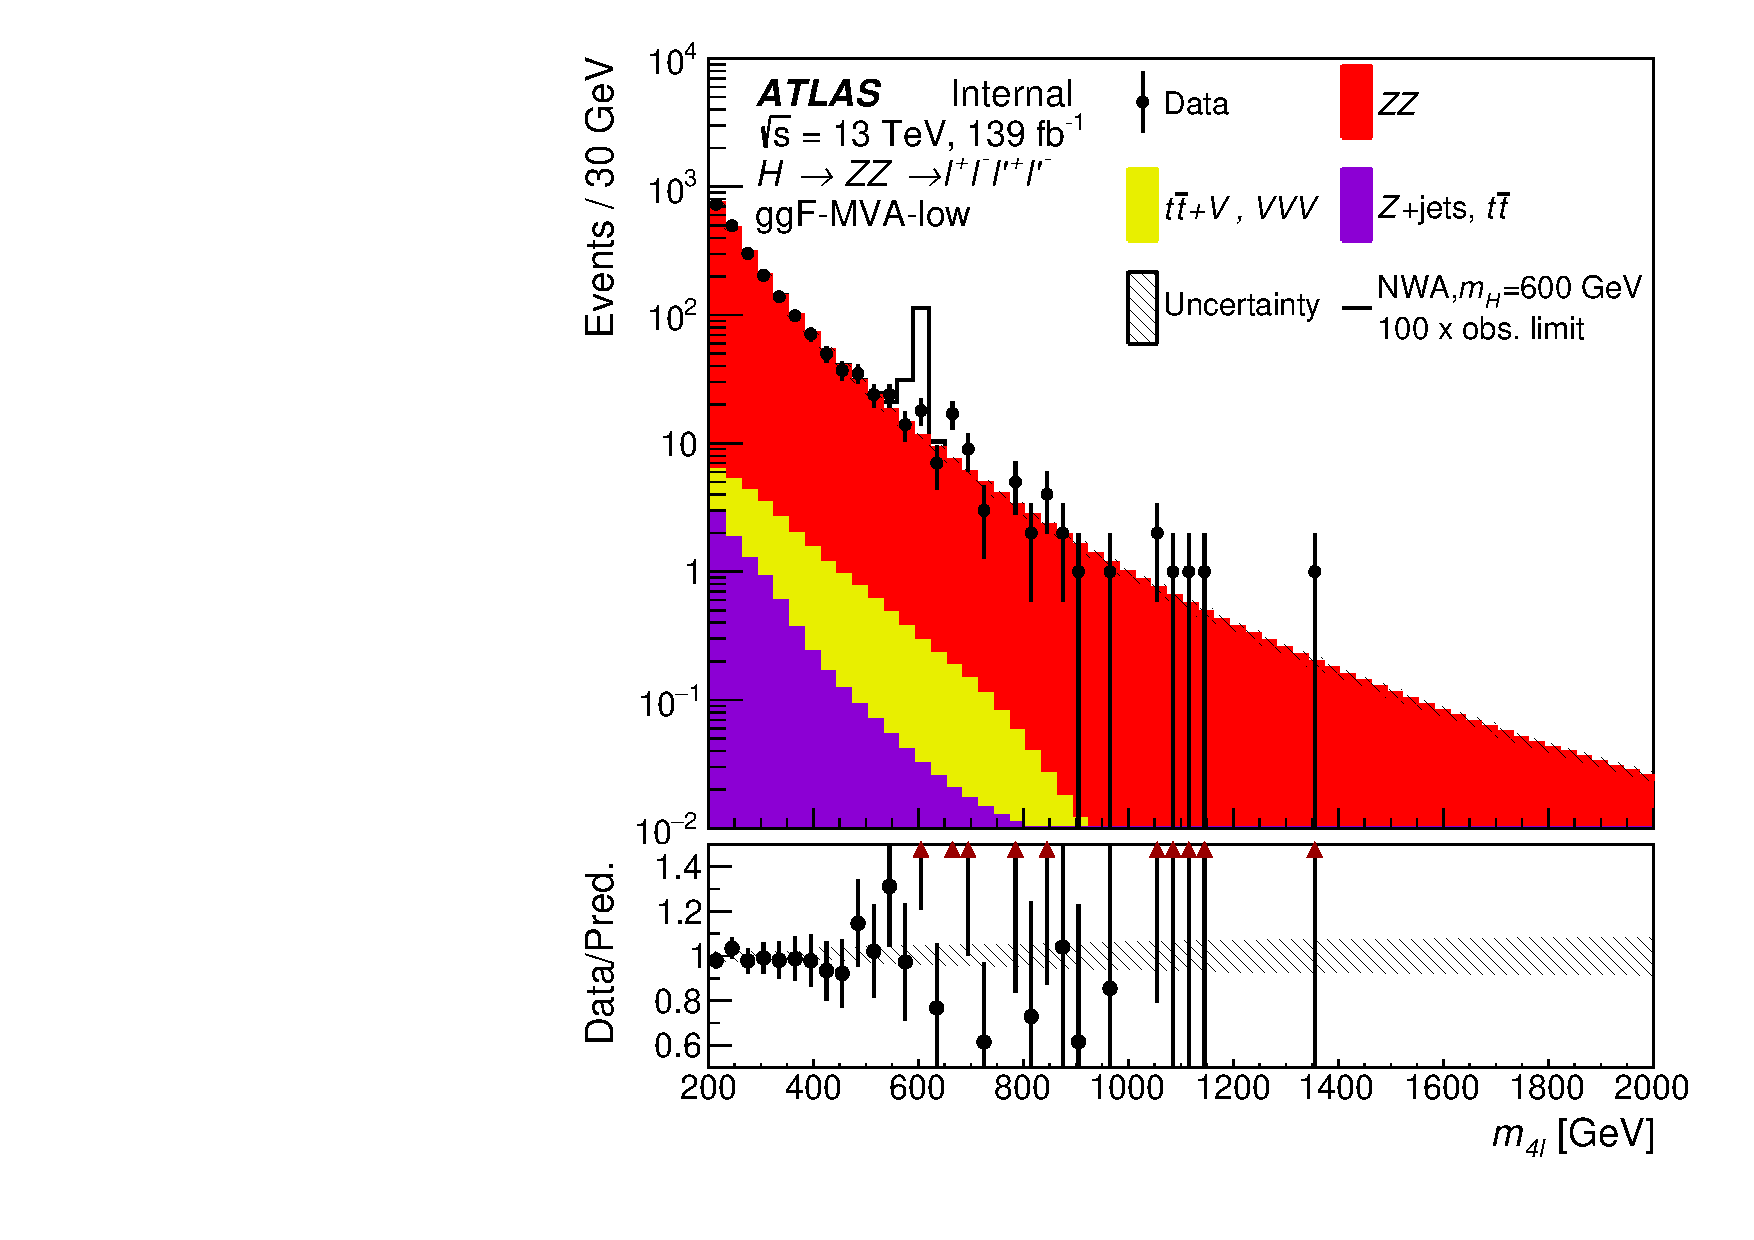
\includegraphics[width=0.32\textwidth]{figures/HMHZZ/results/4l_postfit_m4l_rest_incl.pdf}}
  \subfloat[]{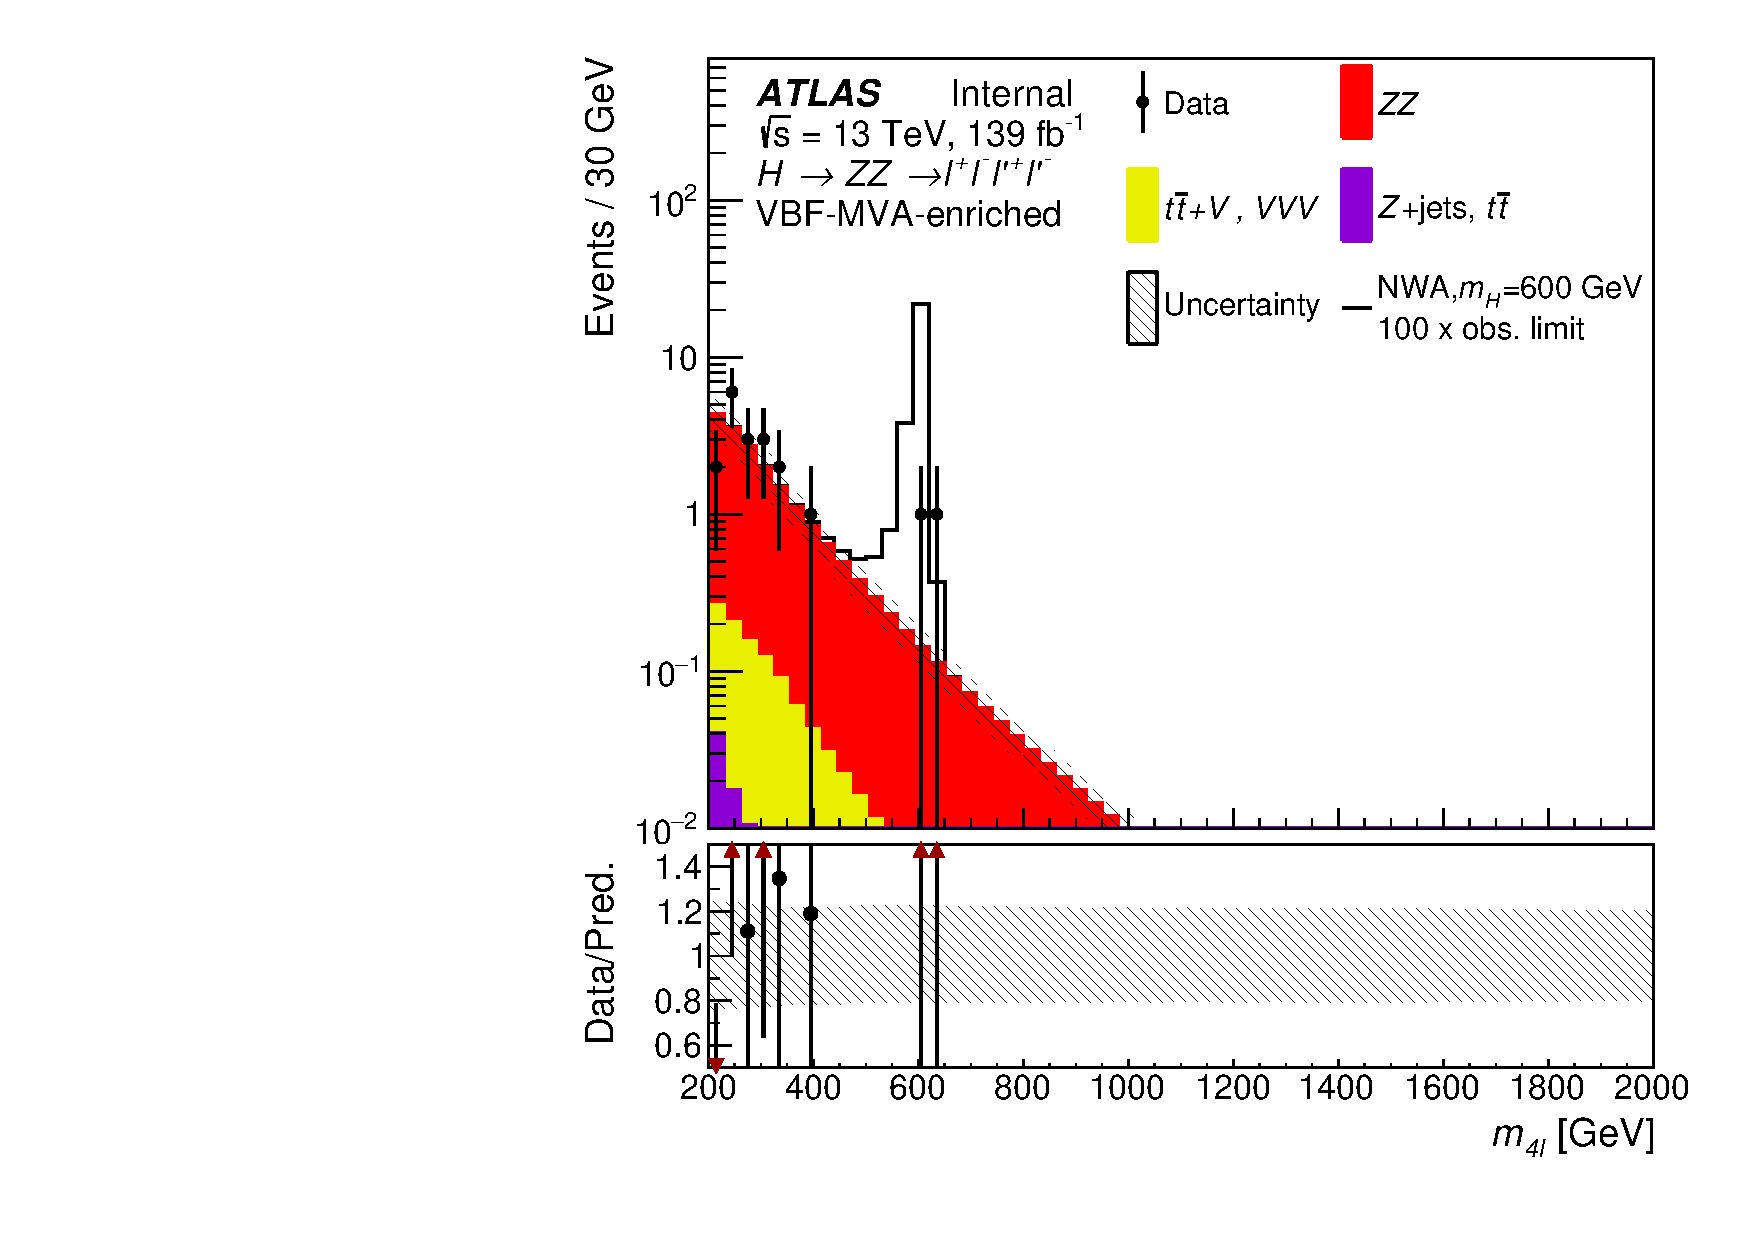
\includegraphics[width=0.32\textwidth]{figures/HMHZZ/results/4l_postfit_m4l_VBF_incl.pdf}}
  
    \caption{Distribution of the four-lepton invariant mass \mfl in the \llll search 
        for (a), (b), (c) the ggF-MVA-high categories, (d) the ggF-MVA-low category 
        and (e) the VBF-MVA-enriched category. 
    The backgrounds are determined from a combined likelihood fit to the data under the background-only 
    hypothesis. The simulated signal at 600~\gev~ is normalized to 
    a cross section corresponding to one hundred times the observed upper limit given in section~\ref{sec:hmhzz_spin0nwa}. 
    The error bars on the data points indicate the statistical uncertainty, 
    while the systematic uncertainty in the prediction is shown by the hatched band. 
    The lower panels show the ratio of data to prediction.}   
  \label{fig:m4l_postfit} 
  \end{center}
\end{figure}


To inspect the likelihood model, pulls and constraints as well as the correlation matrix of NPs are studied by performing a background only fit.
Figure~\ref{fig:NPpull_cb_asimov} shows the pulls and constraints when fitting to pseudo-data (top) and observed data (bottom).
Figure~\ref{fig:NPcorr_cb_asimov} shows the correlation matrix, only for NPs with correlation between each others greater than 0.1 when fitting to pseudo-data.
The normalization of $ZZ$ background is taken from data for one category each, as shown in table~\ref{tab:muZZ_bonly_dnn}.

\begin{table}[htbp]
  \centering
  \caption{$ZZ$ normalization factor in each category, obtained from a likelihood fit to the data under the background-only hypothesis.}
  \label{tab:muZZ_bonly_dnn}
  \small
  \begin{spacing}{1.0}
  \begin{tabular}{ccc}
    \toprule
    Normalization factor  & Fitted value \\
    \midrule
    $\mu_{ZZ}^{ggF-MVA-high}$  & 1.07 $\pm$ 0.047 \\
    \hline
    $\mu_{ZZ}^{ggF-MVA-low}$   & 1.12 $\pm$ 0.026 \\
    \hline
    $\mu_{ZZ}^{VBF-MVA-enriched}$  & 0.91 $\pm$ 0.314 \\
    \bottomrule
  \end{tabular}
  \end{spacing}
\end{table}

\begin{figure}[!ht]
\begin{center}
\subfloat[]{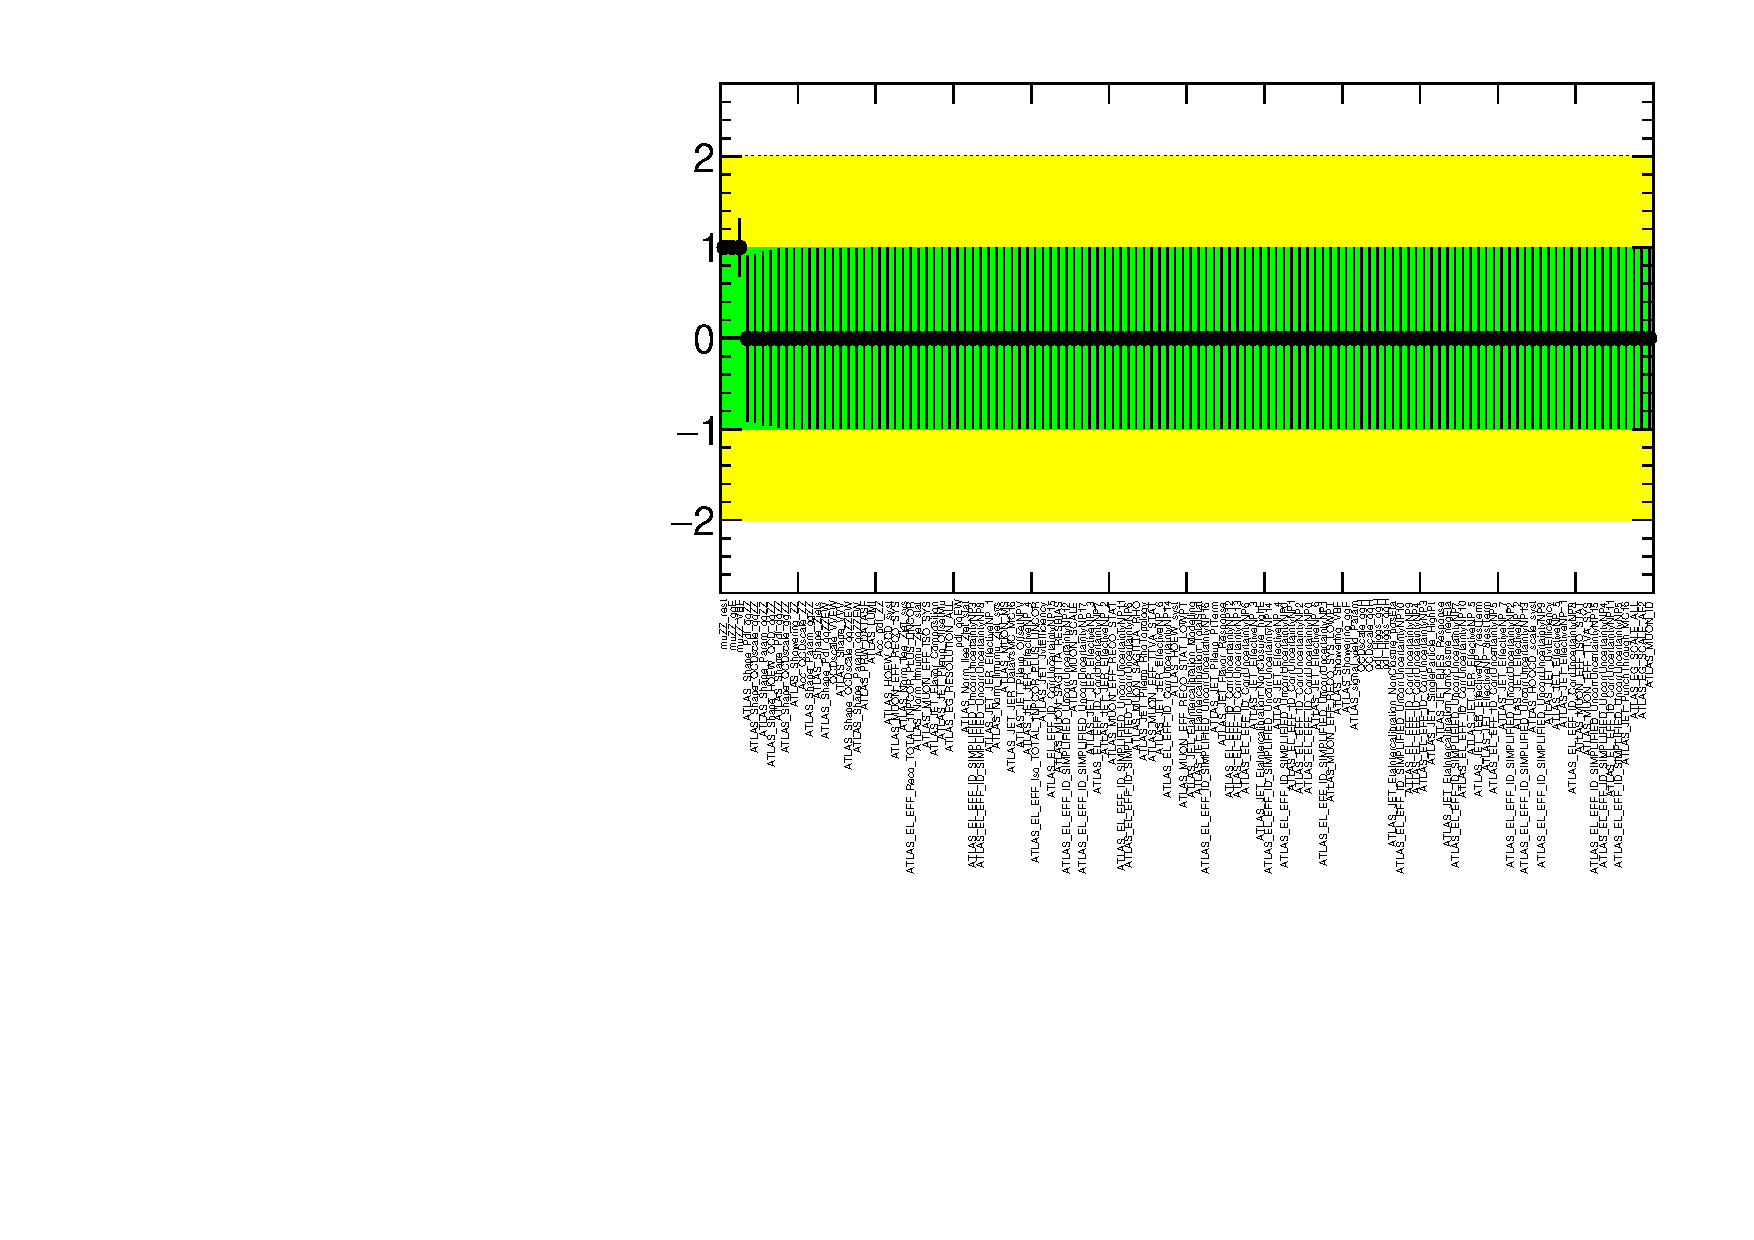
\includegraphics[width=0.8\figwidth]{figures/HMHZZ/results/Pulls_NWA_floatZZ_dnn_Asimov.pdf}}\\
\subfloat[]{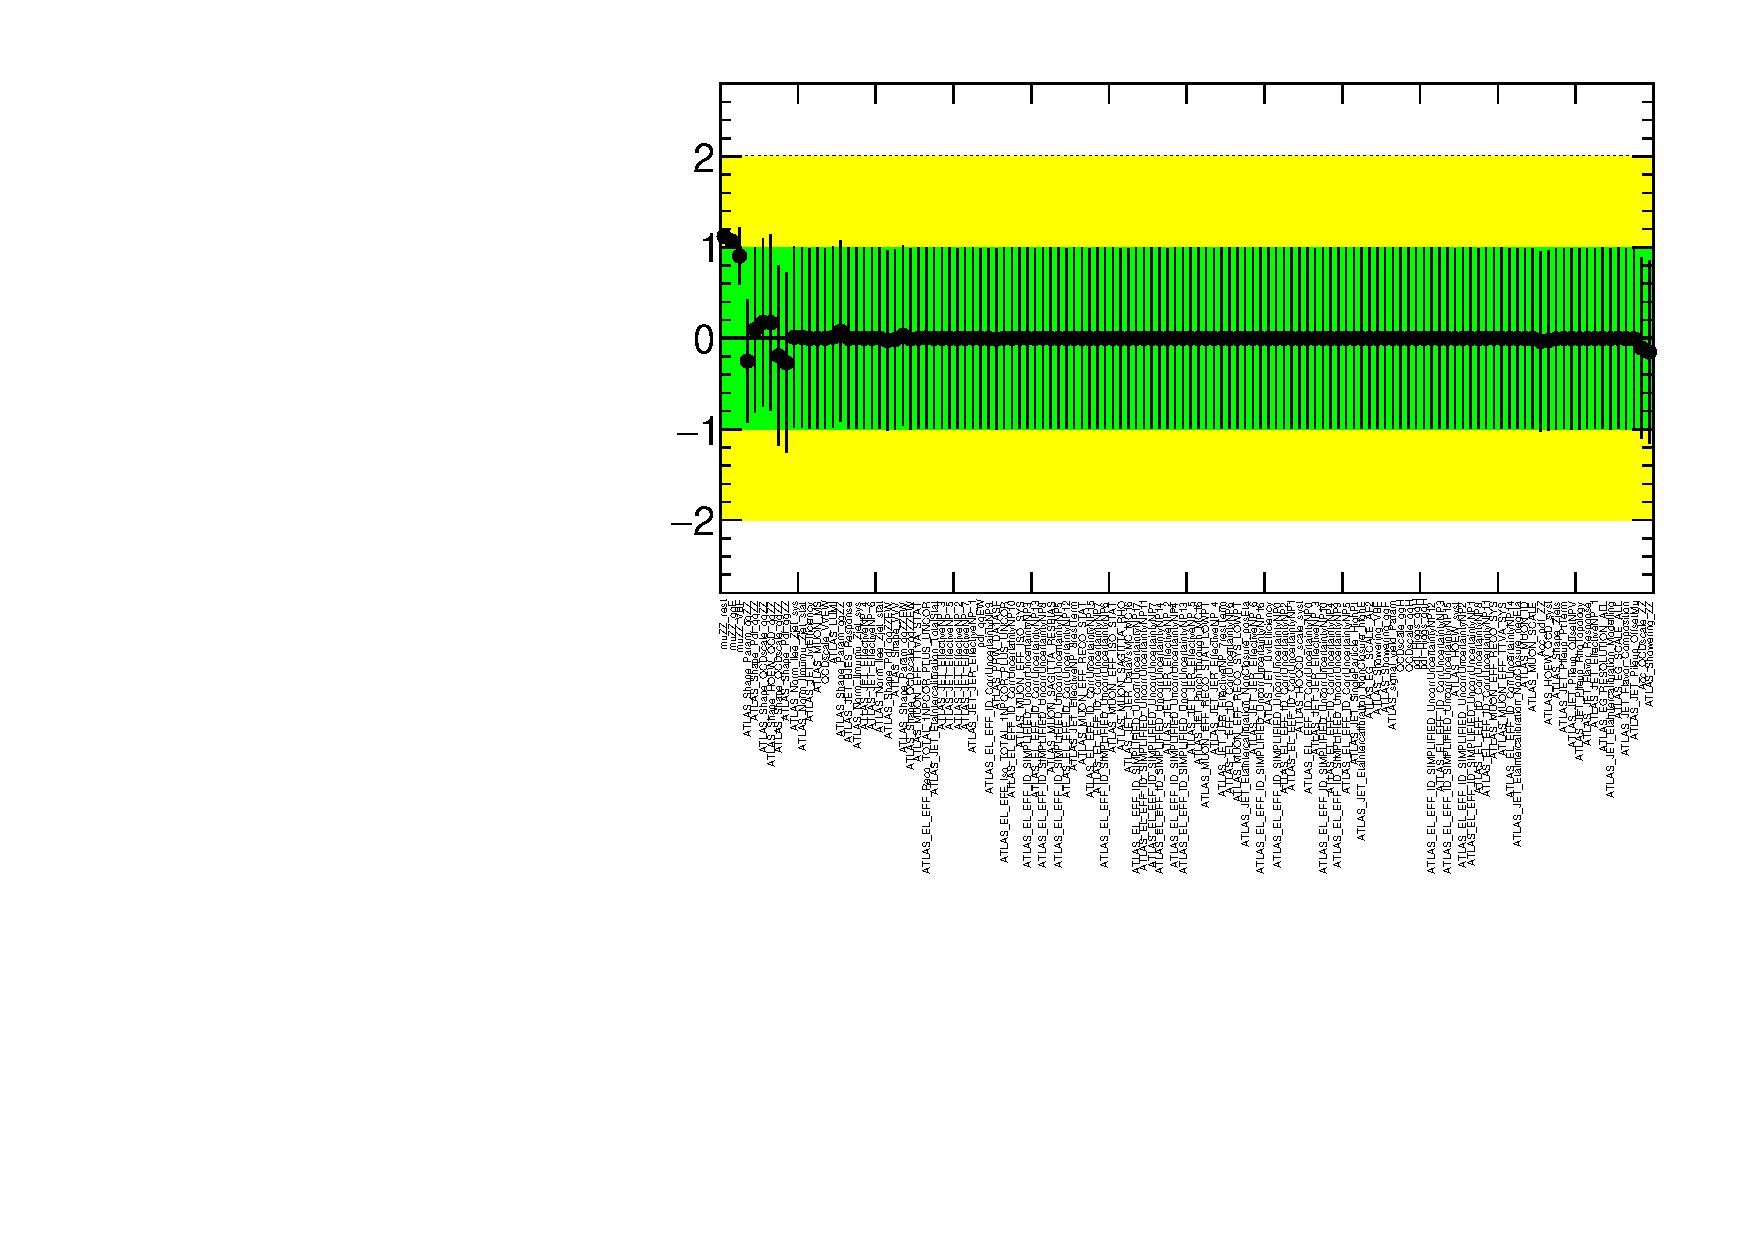
\includegraphics[width=0.8\figwidth]{figures/HMHZZ/results/Pulls_NWA_floatZZ_dnn_Obs.pdf}}
\caption{Pulls and constraints of nuisance parameters after a background only fit to (a) Asimov data and (b) observed data in the \llll channel.
The Asimov data is generated with background data only, and the observed data includes datasets from 2015 to 2018.
}
\label{fig:NPpull_cb_asimov}
\end{center}
\end{figure}

\begin{figure}[!ht]
\begin{center}
\subfloat[]{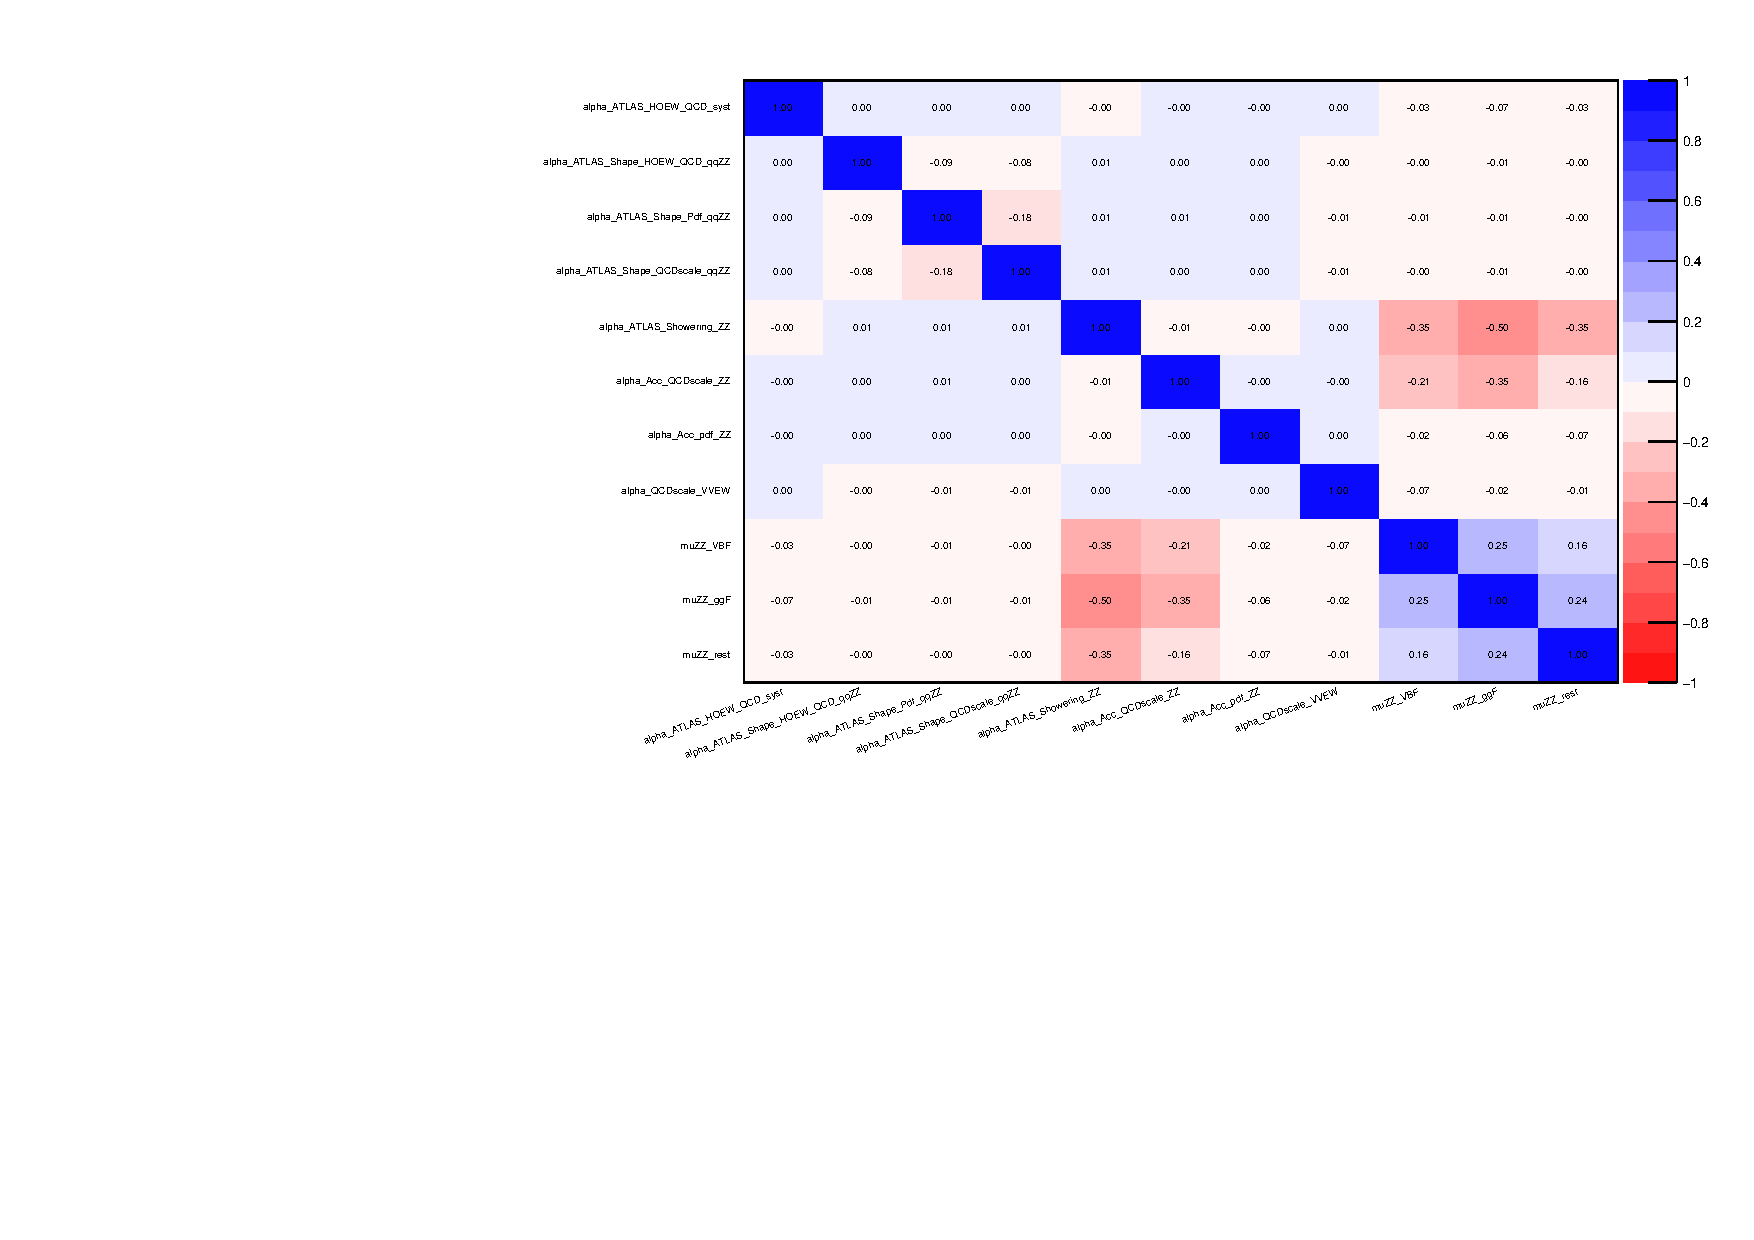
\includegraphics[width=0.8\figwidth]{figures/HMHZZ/results/Correlation_NWA_floatZZ_dnn_Asimov.pdf}}
\caption{Correlation of nuisance parameters after a background only fit to Asimov data in the \llll channel.
The Asimov data is generated with background data only.
}
\label{fig:NPcorr_cb_asimov}
\end{center}
\end{figure}

The impact of a systematic uncertainty on the result depends on the production mode and the mass hypothesis.
To check the impact of systematic uncertainties on expected signal sensitivity, a NP ranking study is performed using
signal injected Asimov data with the injected cross section close to 95\% CLs upper limit at the masses of 400~\gev~ and 1000~\gev.
%The results are shown in Fig.~\ref{fig:rank_cb_NWA_ggF} (\ref{fig:rank_cb_NWA_VBF}) for ggF (VBF) production mode.
The results are shown in table~\ref{tab:NPranking_NWA}.
For ggF production, at lower masses, the systematic uncertainties of parton showering variation for signal, the luminosity uncertainty, 
and the parametrization of signal acceptance dominate,
while at higher masses, the shape uncertainties from PDF variation for ZZ (\qqZZ and \ggZZ) background become important, as also seen in VBF production mode.
In addition for VBF, jet related uncertainties become more important comparing to ggF production.
Moreover, the dominate uncertainties include the acceptance uncertainty from QCD scale variation for signal and the luminosity uncertainty.

\begin{table}[htbp!]
    \caption{\label{tab:NPranking_NWA}
    Impact of the leading systematic uncertainties, the data statistic uncertainties,
    as well as the total uncertainties on the
    predicted signal event yield with the cross section times branching ratio being 
    set to the expected upper limit, 
    expressed as a percentage of the signal yield
    for the ggF (left) and VBF (right) production modes at $\mH = 400$ and $1000~\gev$.
    }
    %\footnotesize
    \centering
    \begin{tabular}{l l | l l}
      \toprule
      \multicolumn{2}{c|}{ggF production} &  \multicolumn{2}{c}{VBF production} \\
      \multicolumn{2}{l|}{Systematic source    \hfill Impact [\%]}   & \multicolumn{2}{l}{Systematic source \hfill Impact [\%]}\\
      \midrule
      \multicolumn{4}{c}{$\bigstrut$  $\mH=400~\gev$}\\
      \midrule

       Parton showering of ggF       & 2.3 & QCD scale of VBF                     & 2.7 \\
       Luminosity                    & 1.8 & Jet flavor composition               & 2.5 \\
       PDF of \qqZZ                  & 1.6 & Luminosity                           & 1.8 \\
       Signal yield parameterization & 1.4 & Jet energy scale (in-su calibration) & 1.6 \\
      Data stat. uncertainty         &  48 & Data stat. uncertainty               & 57 \\
      Total Uncertainty              &  49 & Total Uncertainty                    & 58 \\
      \midrule
      \multicolumn{4}{c}{$\bigstrut$  $\mH=1000~\gev$}\\
      \midrule

       PDF of \qqZZ              & 2.5 & QCD scale of VBF       & 2.3 \\
       Parton showering of ggF   & 2.4 & PDF of \qqZZ           & 2.2 \\
       PDF of \ggZZ              & 1.9 & Luminosity             & 1.8 \\
       Luminosity                & 1.8 & PDF of \ggZZ           & 1.6 \\
      Data stat. uncertainty     &  84 & Data stat. uncertainty & 92 \\        
      Total Uncertainty          &  86 & Total Uncertainty      & 93 \\
      \bottomrule

    \end{tabular}
  \end{table}

%\begin{figure}[!ht]
%\begin{center}
%\subfloat[]{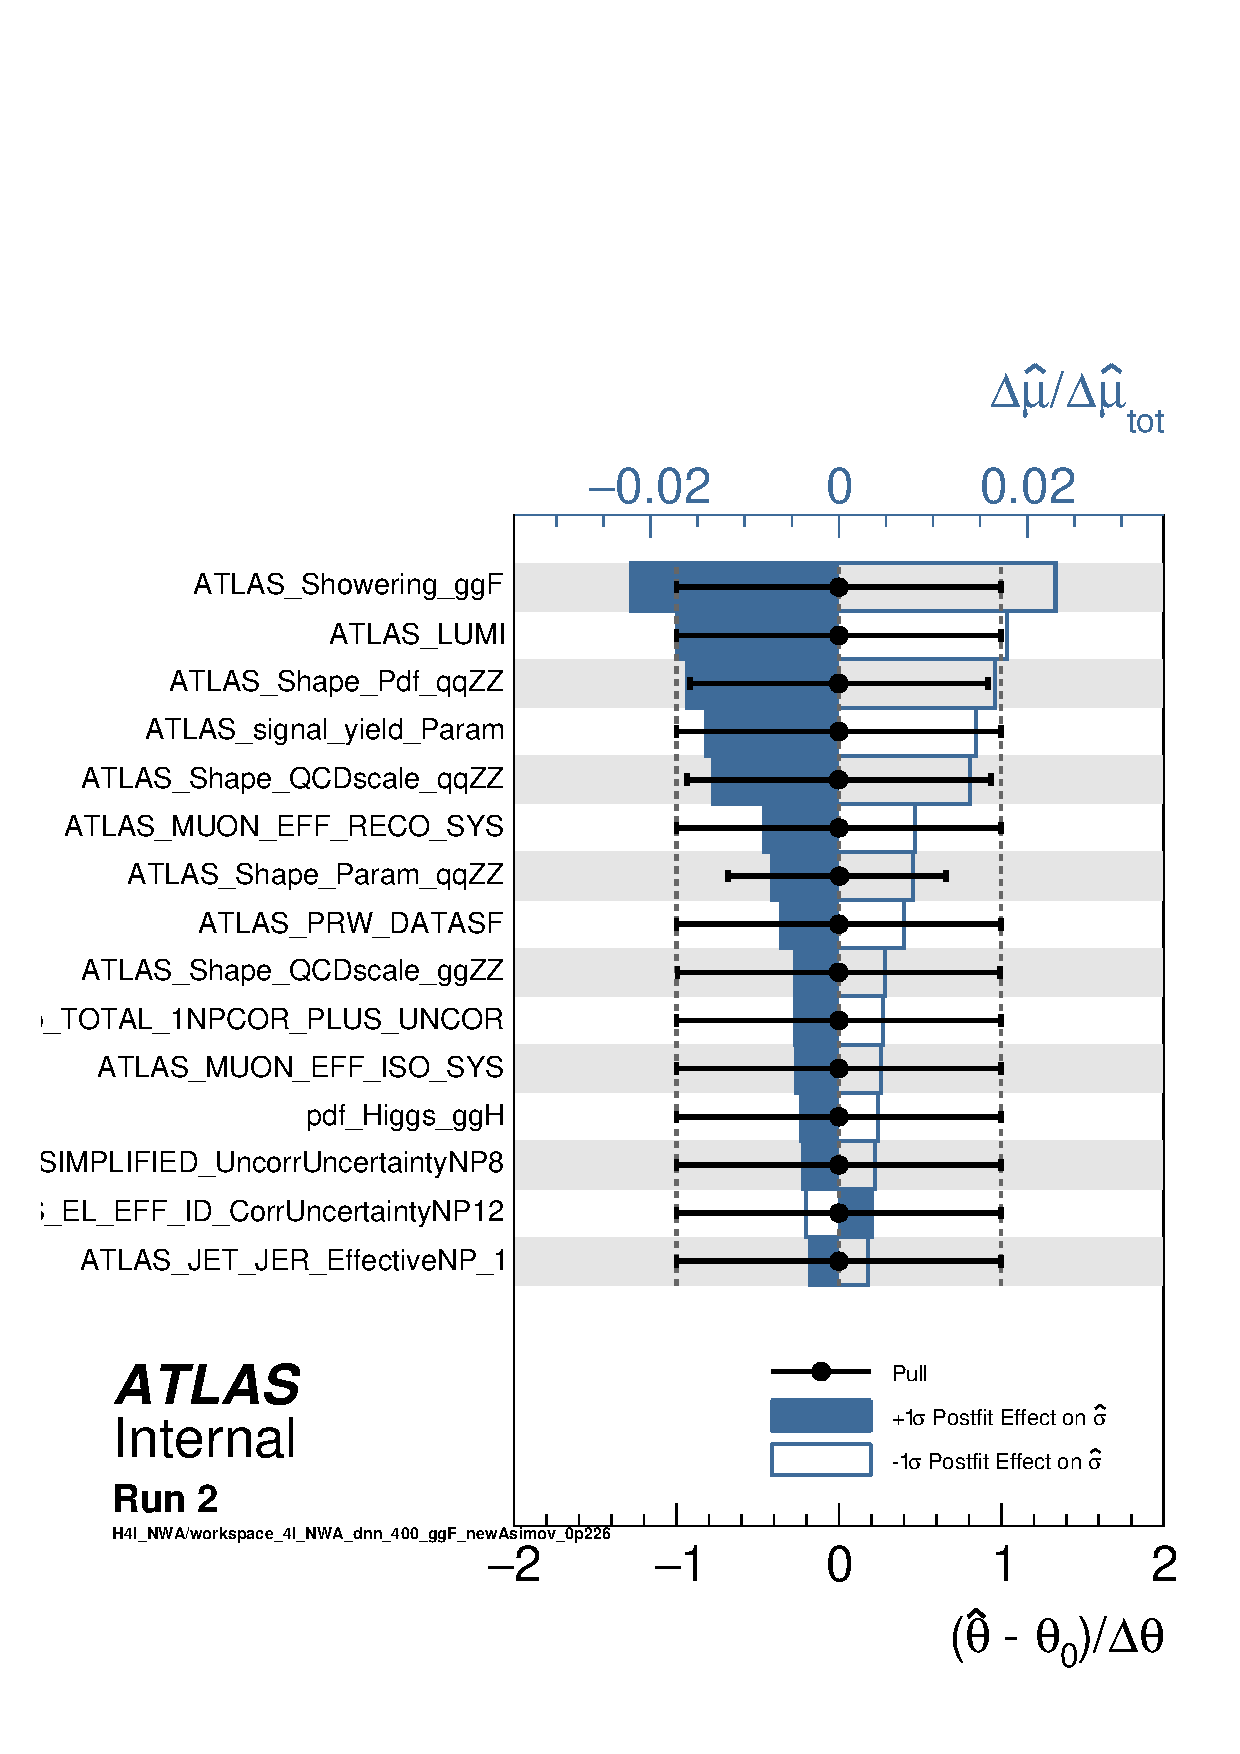
\includegraphics[width=0.48\figwidth]{figures/HMHZZ/results/workspace_4l_NWA_dnn_400_ggF_newAsimov_0p226_pulls_paper.pdf}}
%\subfloat[]{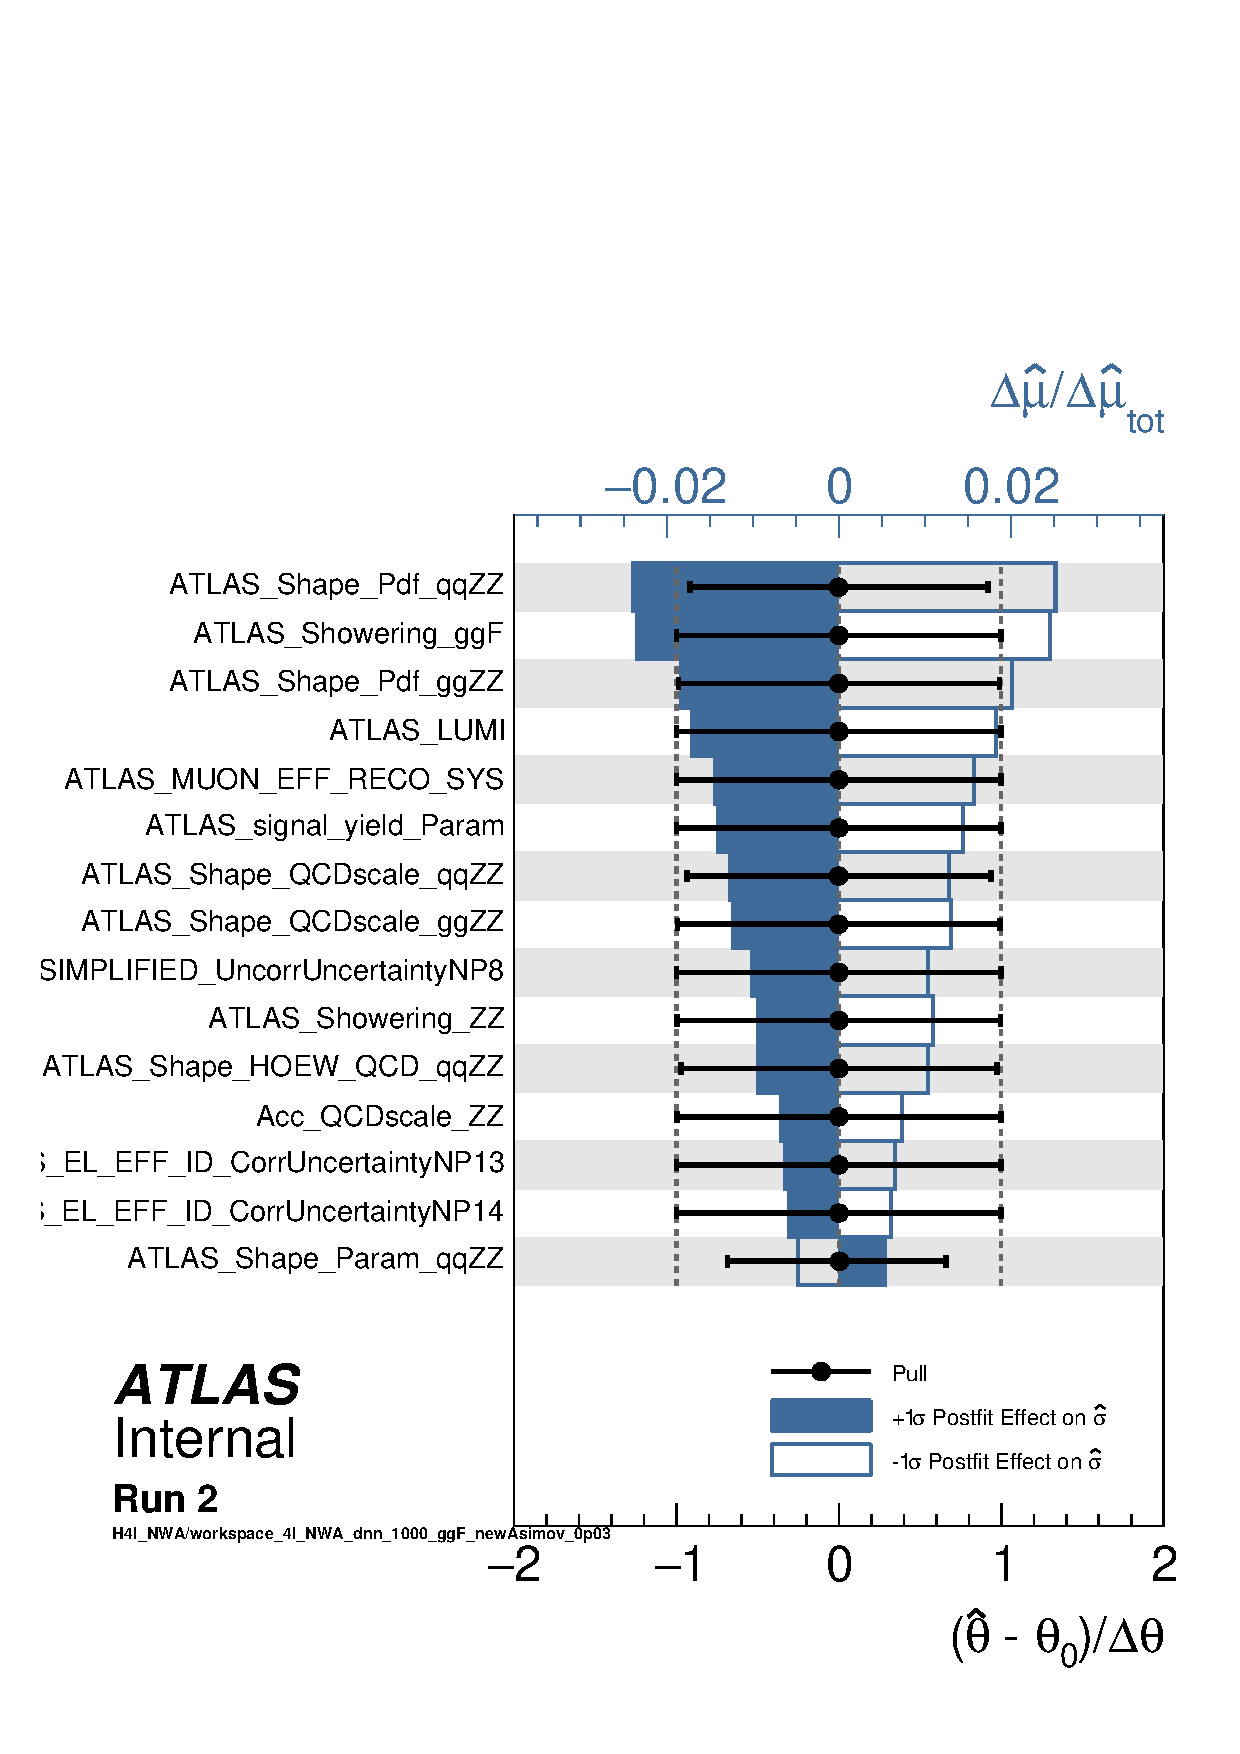
\includegraphics[width=0.48\figwidth]{figures/HMHZZ/results/workspace_4l_NWA_dnn_1000_ggF_newAsimov_0p03_pulls_paper.pdf}}
%\caption{NP ranking plot for the \xsggF\ fit to Asimov data in the \llll channel.
%The Asimov data is injected with \xsggF\ = 0.226 fb for $m_H = 400$ GeV (left) and \xsggF\ = 0.030 fb for $m_H = 1000$ GeV (right).
%}
%\label{fig:rank_cb_NWA_ggF}
%\end{center}
%\end{figure}
%
%\begin{figure}[!ht]
%\begin{center}
%\subfloat[]{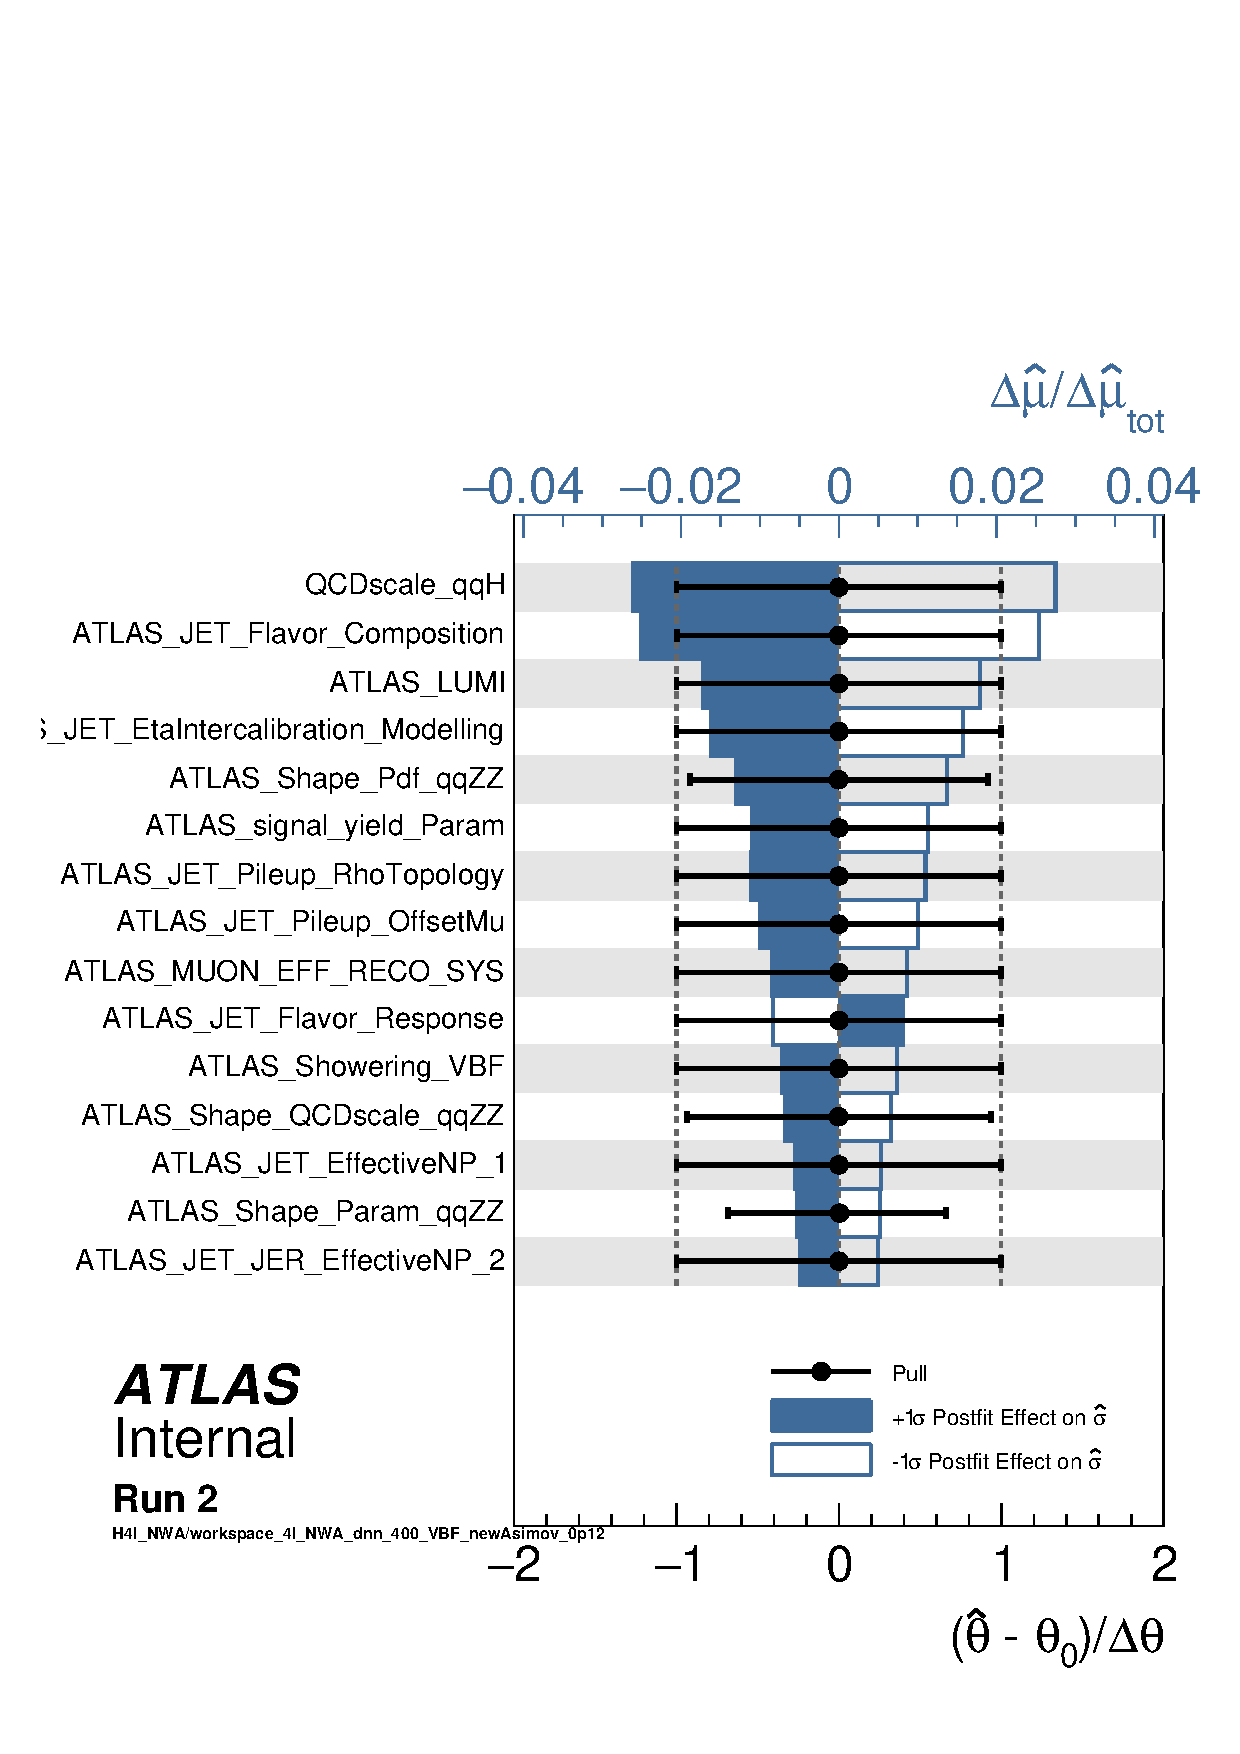
\includegraphics[width=0.48\figwidth]{figures/HMHZZ/results/workspace_4l_NWA_dnn_400_VBF_newAsimov_0p12_pulls_paper.pdf}}
%\subfloat[]{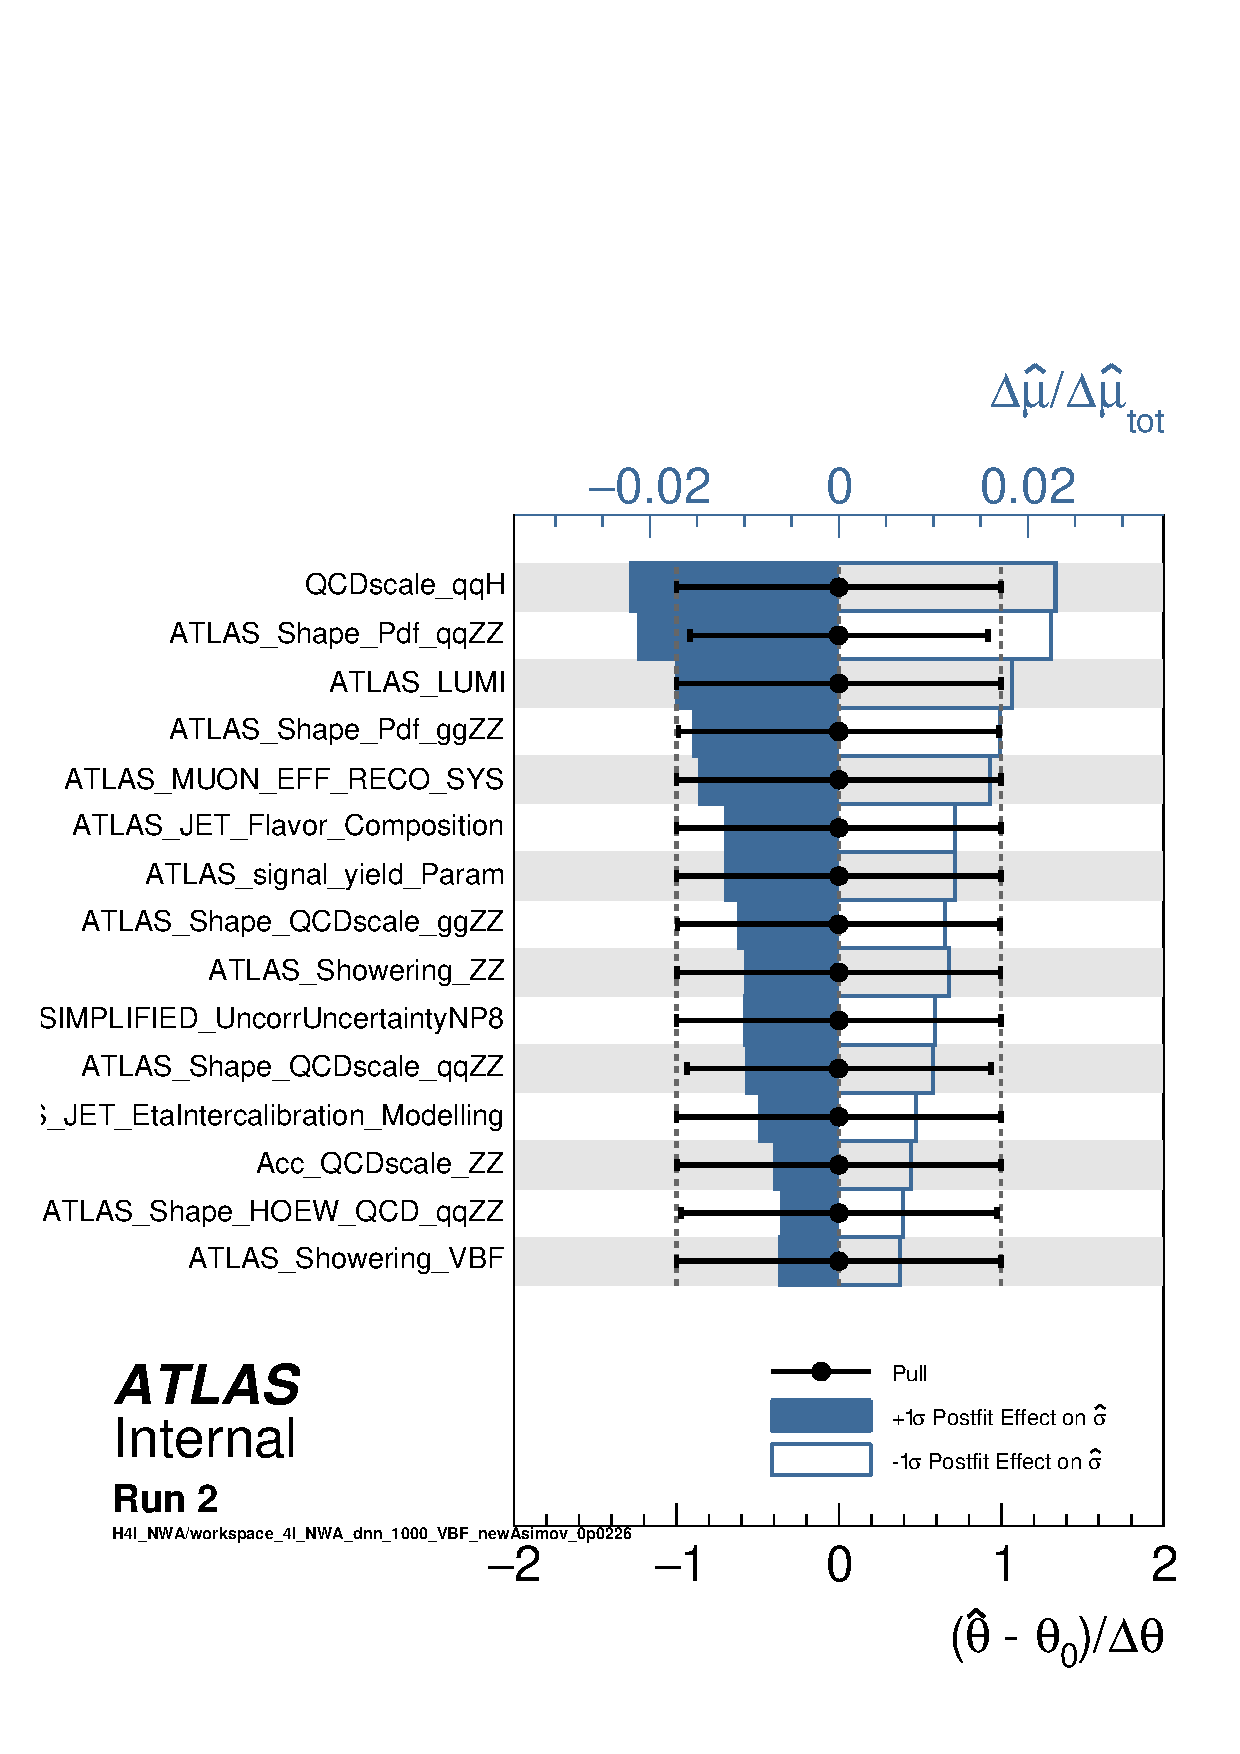
\includegraphics[width=0.48\figwidth]{figures/HMHZZ/results/workspace_4l_NWA_dnn_1000_VBF_newAsimov_0p0226_pulls_paper.pdf}}
%\caption{NP ranking plot for the \xsVBF\ fit to Asimov data in the \llll channel.
%The Asimov data is injected with \xsVBF\ = 0.120 fb for $m_H = 400$ GeV (left) and \xsVBF\ = 0.0226 fb for $m_H = 1000$ GeV (right).
%}
%\label{fig:rank_cb_NWA_VBF}
%\end{center}
%\end{figure}


%% =======================================================================================================
\subsection{Interpretations}
\label{sec:hmhzz_spin0nwa}

\subsubsection{Spin-0 resonance with NWA}

In the absence of a specific model, the ratio of ggF and VBF production mode is unknown for this additional heavy scalar.
For this reason, the fits for ggF and VBF processes are done separately, and in each case the cross section of the untested process is allowed to be a free parameter in the statistical fit.
The observed and expected upper limit at 95\% confidence level (CL) on the $\sigma \times BR(H \rightarrow ZZ)$ of a narrow scalar resonance for both ggF (left) and VBF (right) production mode with the integrated luminosity of \lumi is shown in figure~\ref{fig:NWA201518_MVA} (\ref{fig:NWA201518_Cut}) for MVA- (cut-) based analysis.
No excess over 2$\sigma$ is found.

\begin{figure}[h]
    \centering
    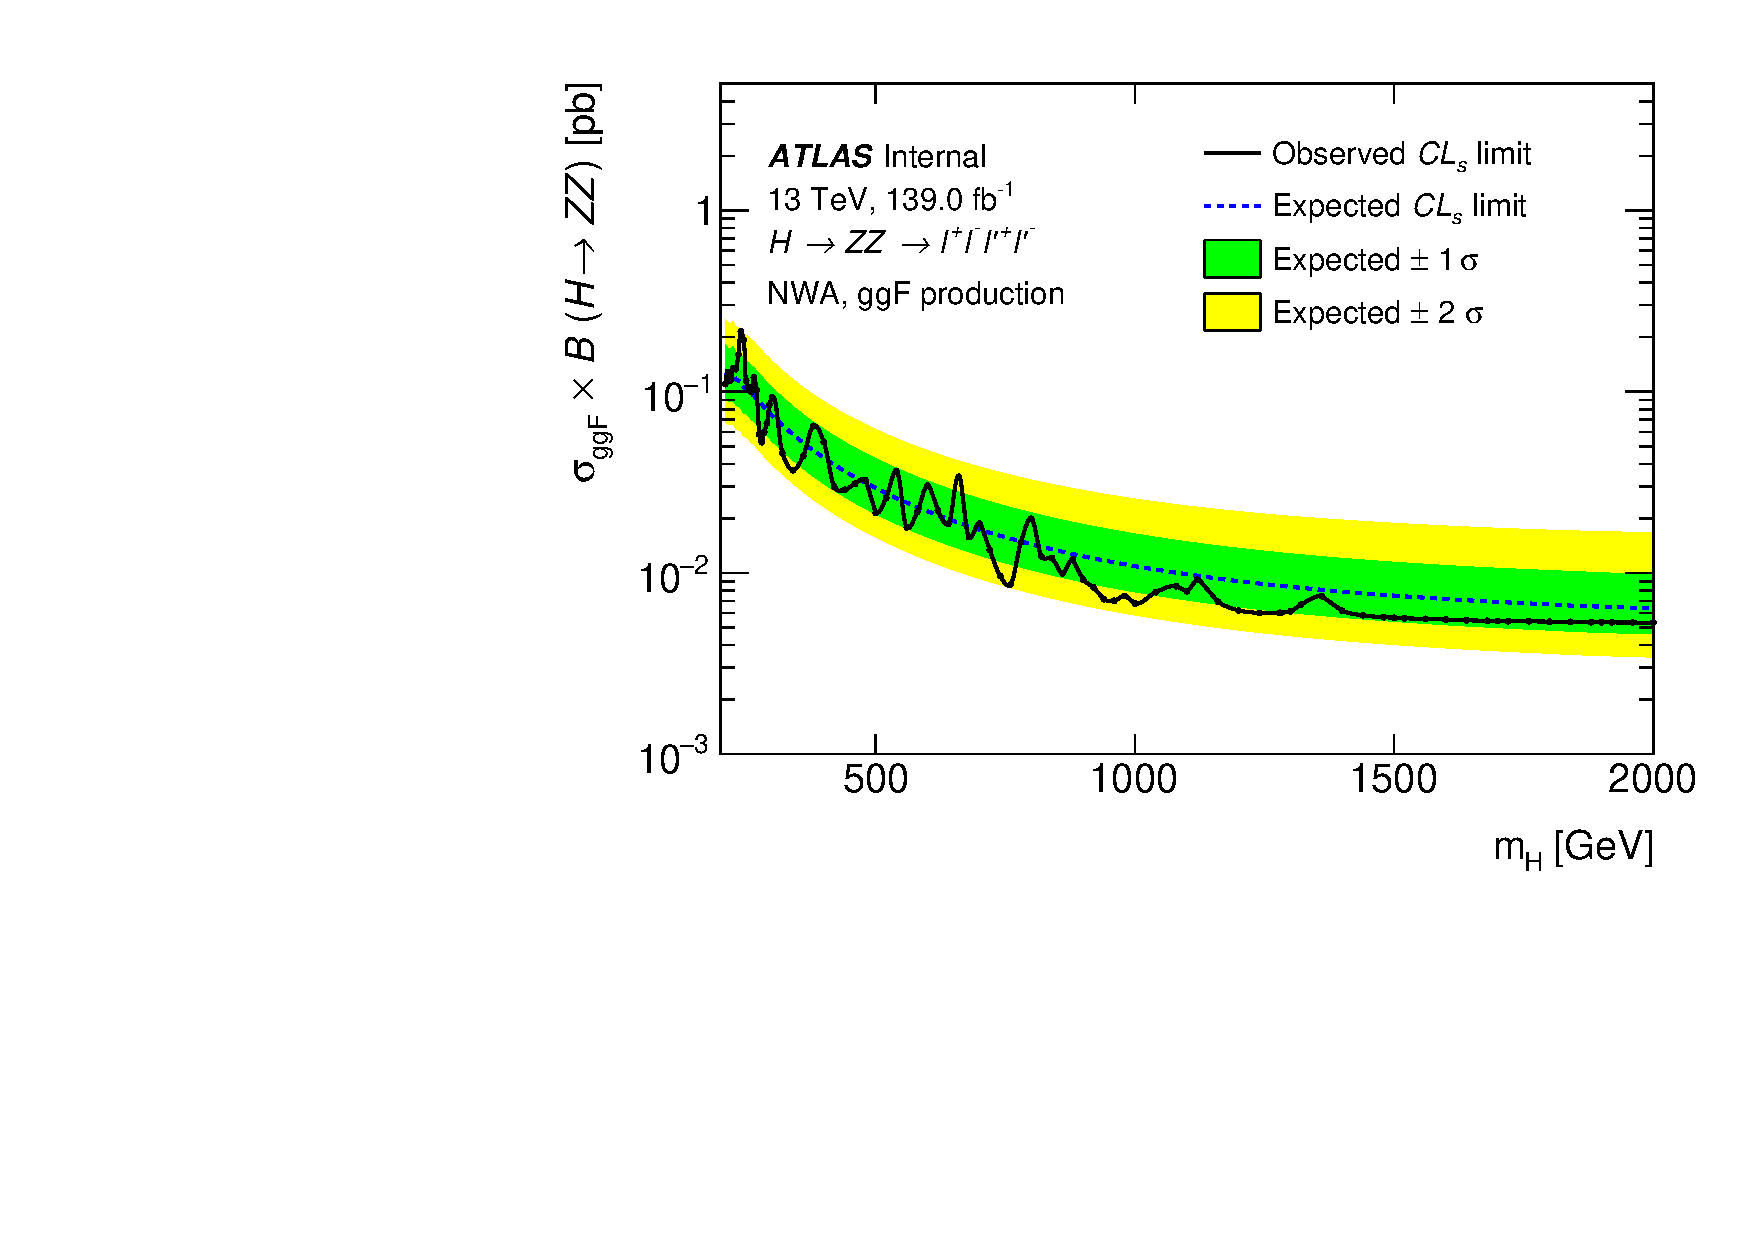
\includegraphics[width=0.48\textwidth]{figures/HMHZZ/results/limits_DNN_ggF.pdf}
    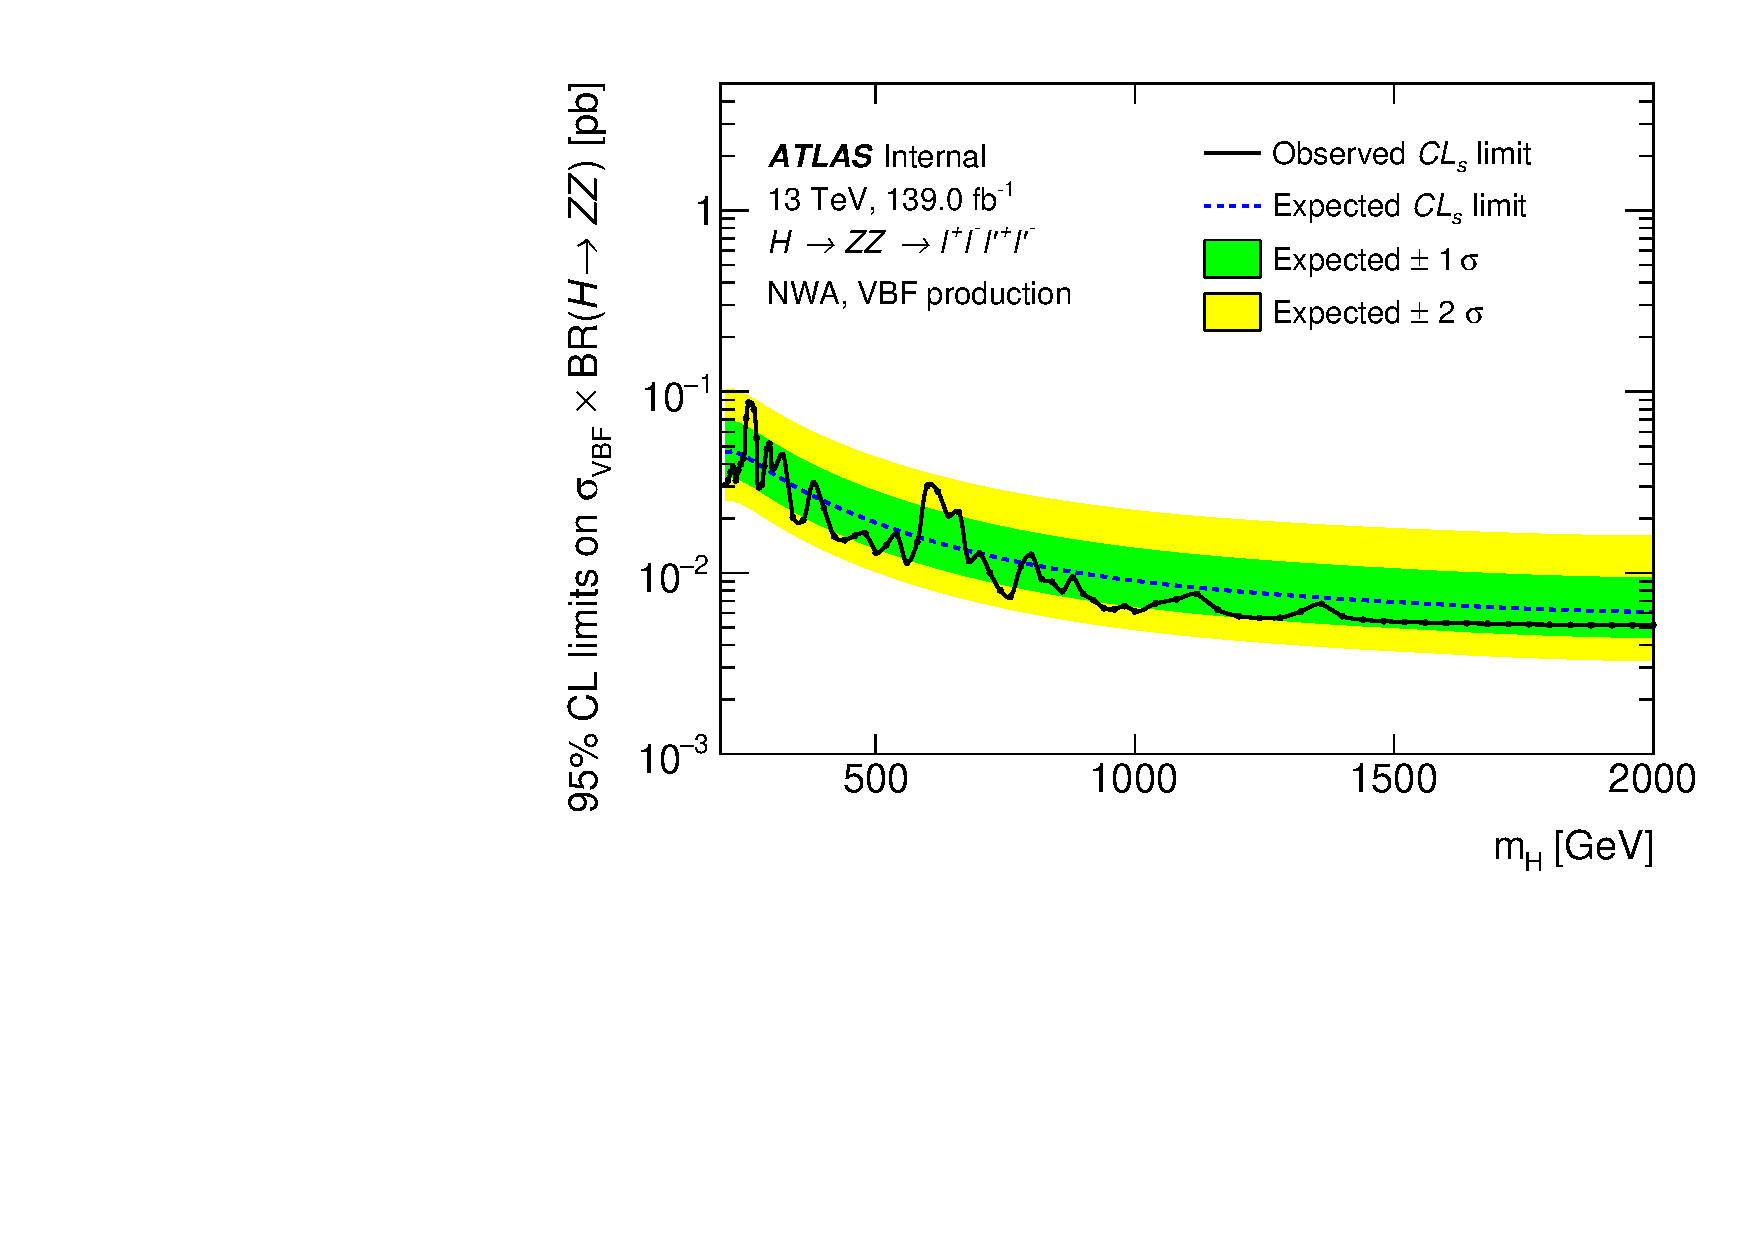
\includegraphics[width=0.48\textwidth]{figures/HMHZZ/results/limits_DNN_VBF.pdf}
    \caption{The expected and observed upper limits at 95\% CL on $\sigma \times BR(H \rightarrow ZZ)$ using the MVA-based analysis for ggF (left) and VBF (right) production. The green and yellow bands represent the $\pm 1\sigma$ and $\pm 2\sigma$ uncertainties in the expected limits.
 }
    \label{fig:NWA201518_MVA}
\end{figure}

\begin{figure}[h]
    \centering
    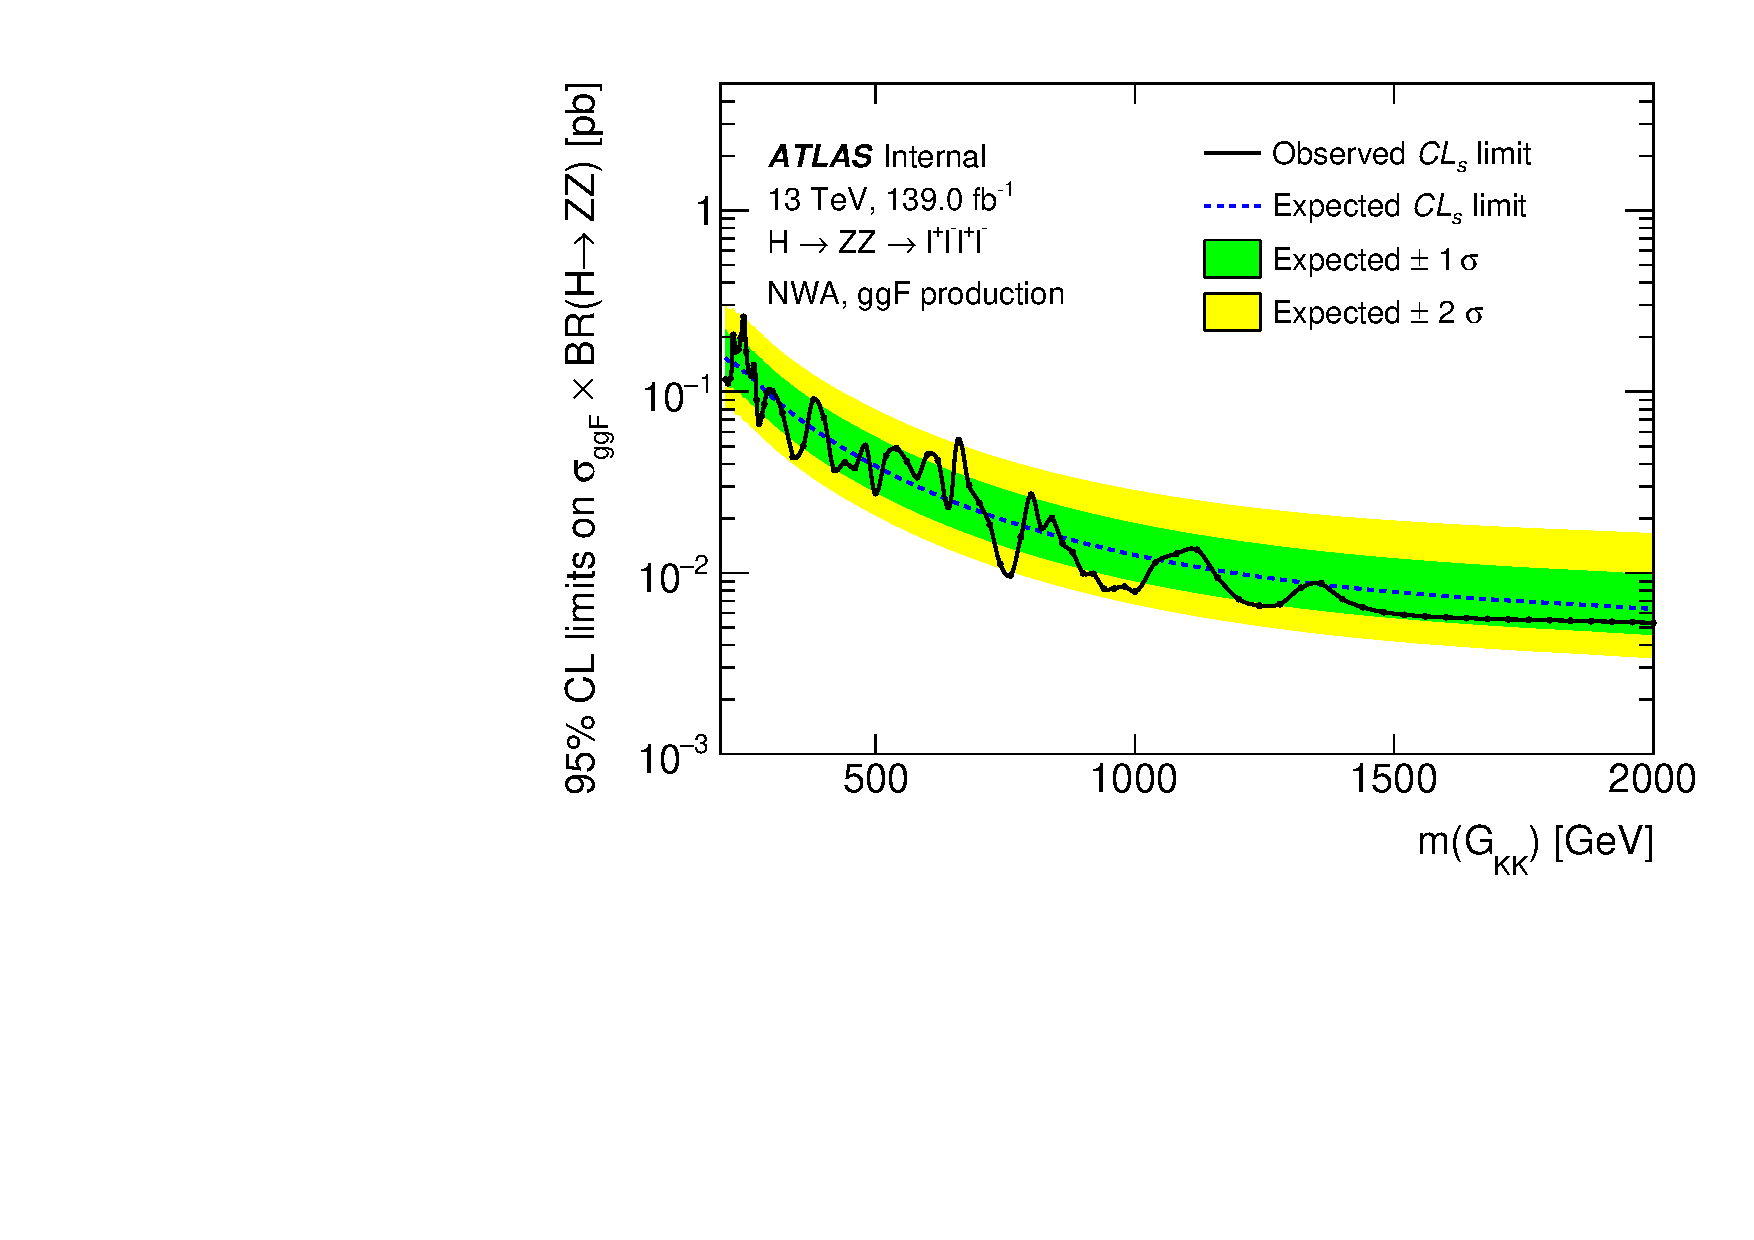
\includegraphics[width=0.48\textwidth]{figures/HMHZZ/results/limits_Cut2020_ggF.pdf}
    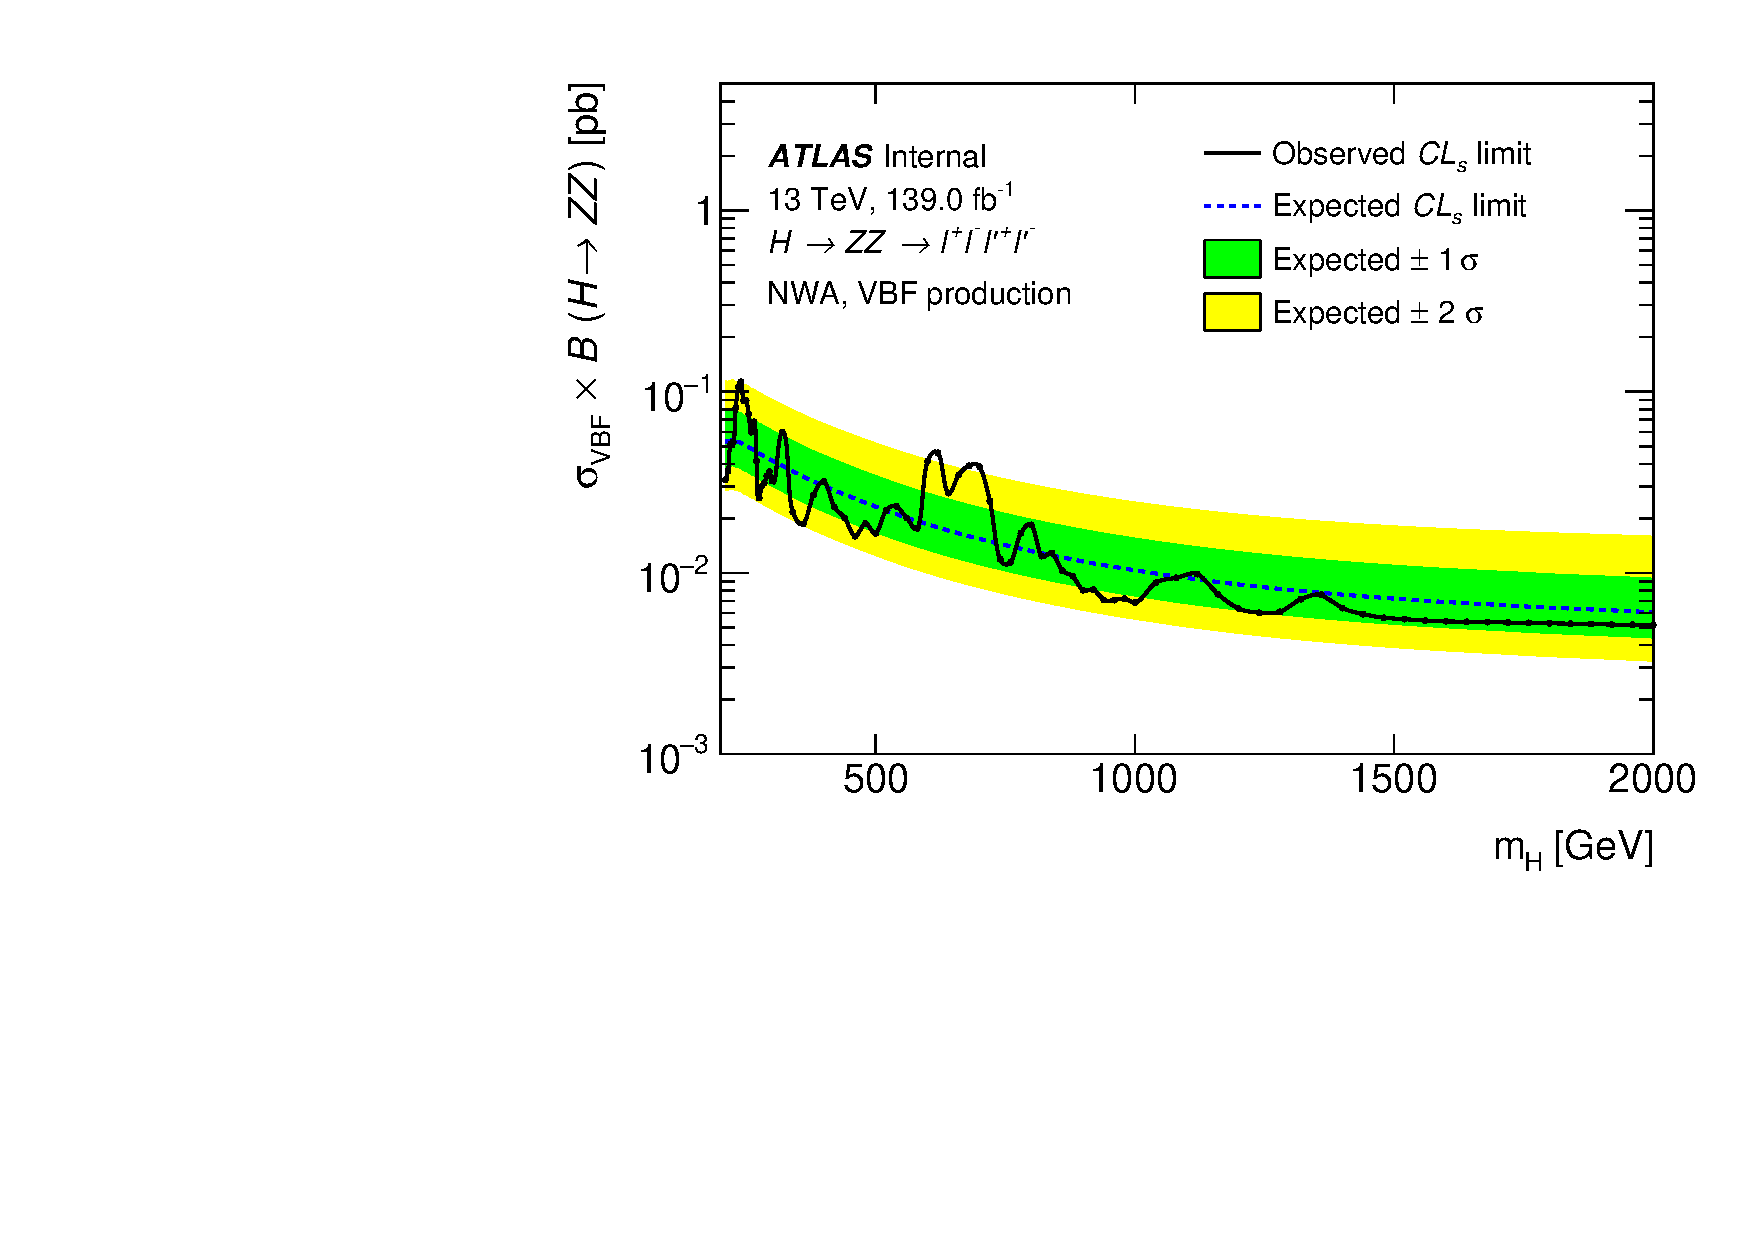
\includegraphics[width=0.48\textwidth]{figures/HMHZZ/results/limits_Cut2020_VBF.pdf}
    \caption{The expected and observed upper limits at 95\% CL on $\sigma \times BR(H \rightarrow ZZ)$ using the cut-based analysis for ggF (left) and VBF (right) production. The green and yellow bands represent the $\pm 1\sigma$ and $\pm 2\sigma$ uncertainties in the expected limits.
 }
    \label{fig:NWA201518_Cut}
\end{figure}

\subsubsection{Spin-0 resonance with LWA}

In the case of LWA model, only ggF production mode is studied.
The interference between the heavy scalar and SM Higgs boson (H-h), as well as the heavy scalar and SM \ggZZ continuum background (H-B) as modelled in section~\ref{sec:int_model} are token into account.
The upper limit at 95\% confidence level (CL) on ggF cross section times branch ratio ($\sigma_{ggF} \times BR(H \rightarrow ZZ)$) is shown in figure~\ref{fig:LWAlimits_ggF_201518_withInt} for a width of 1, 5, 10 and 15\% of \mH.

\begin{figure}[h]
    \begin{center}
    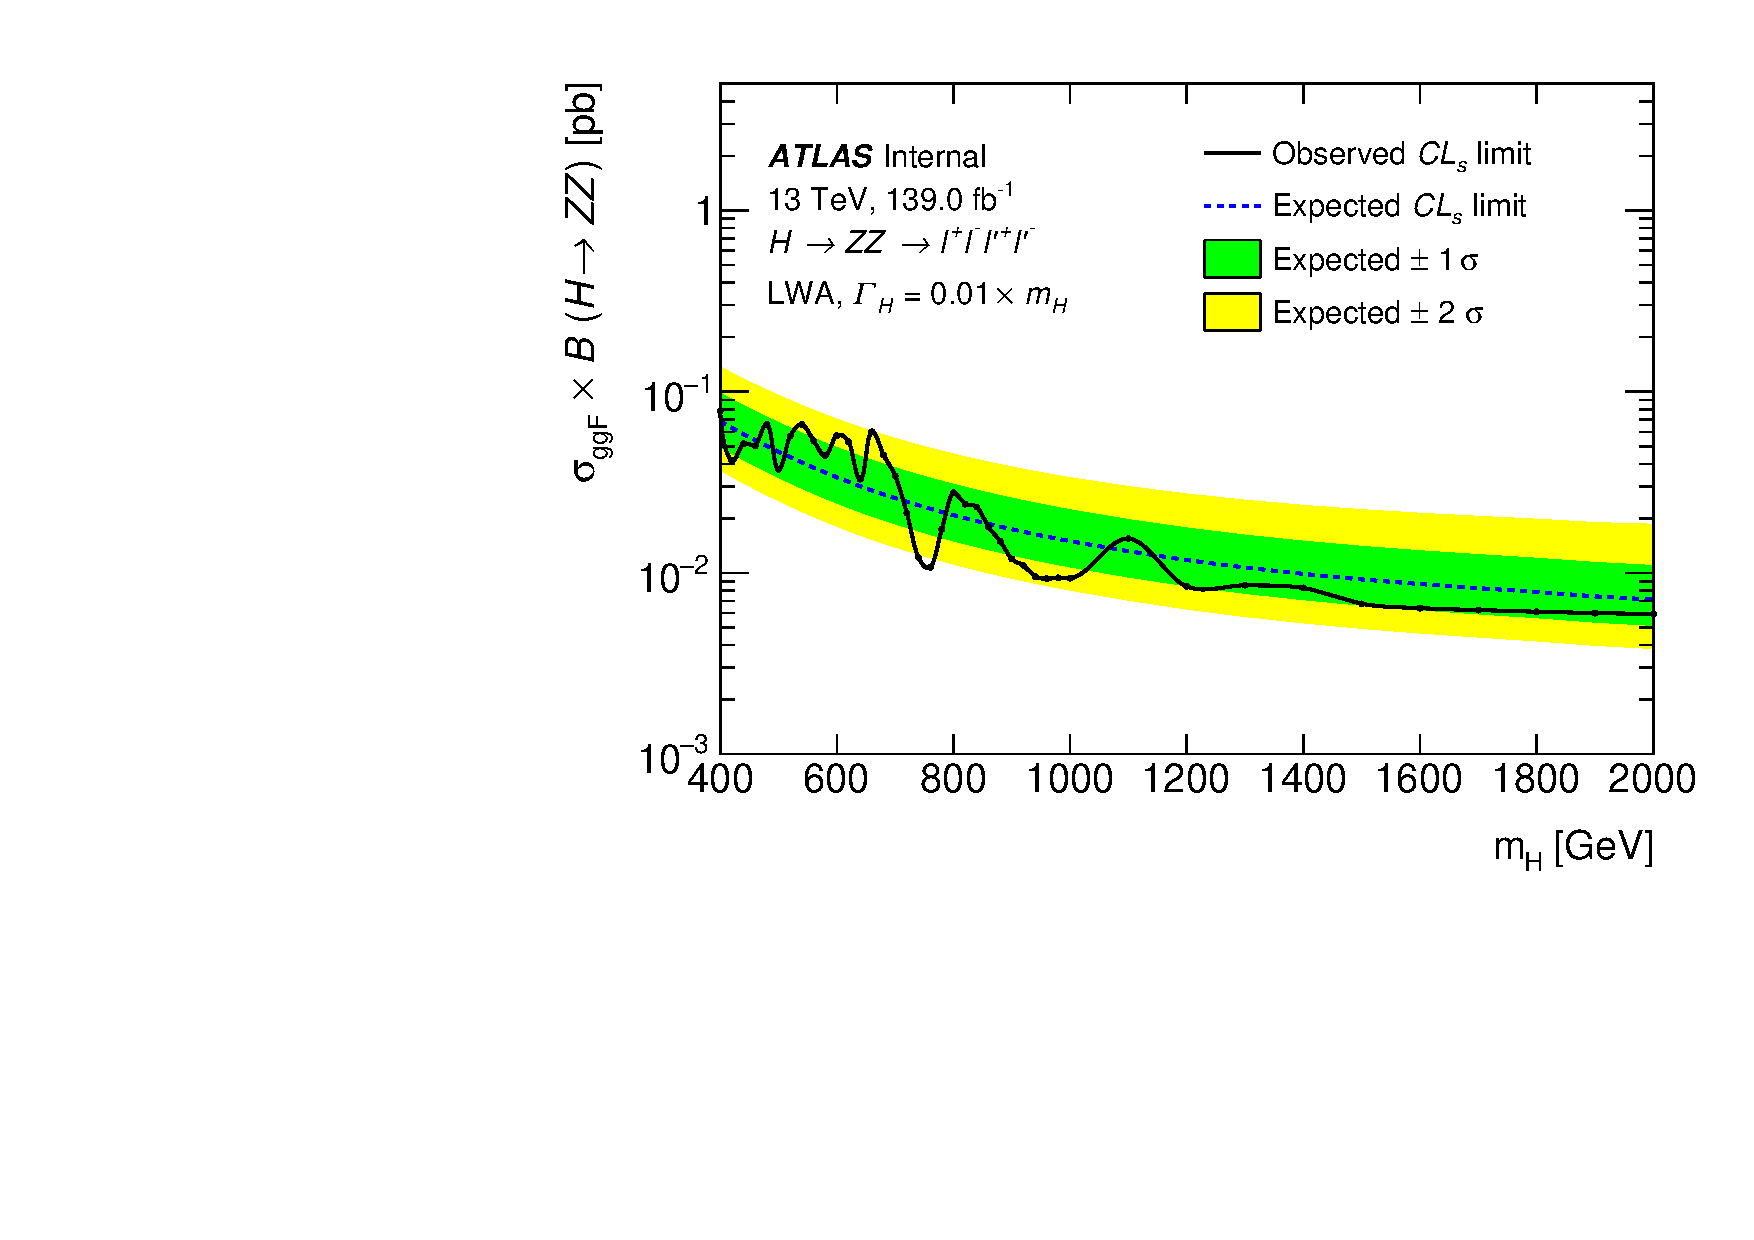
\includegraphics[width=0.48\textwidth]{figures/HMHZZ/results/Limits_LWA_withInt_1.pdf}
    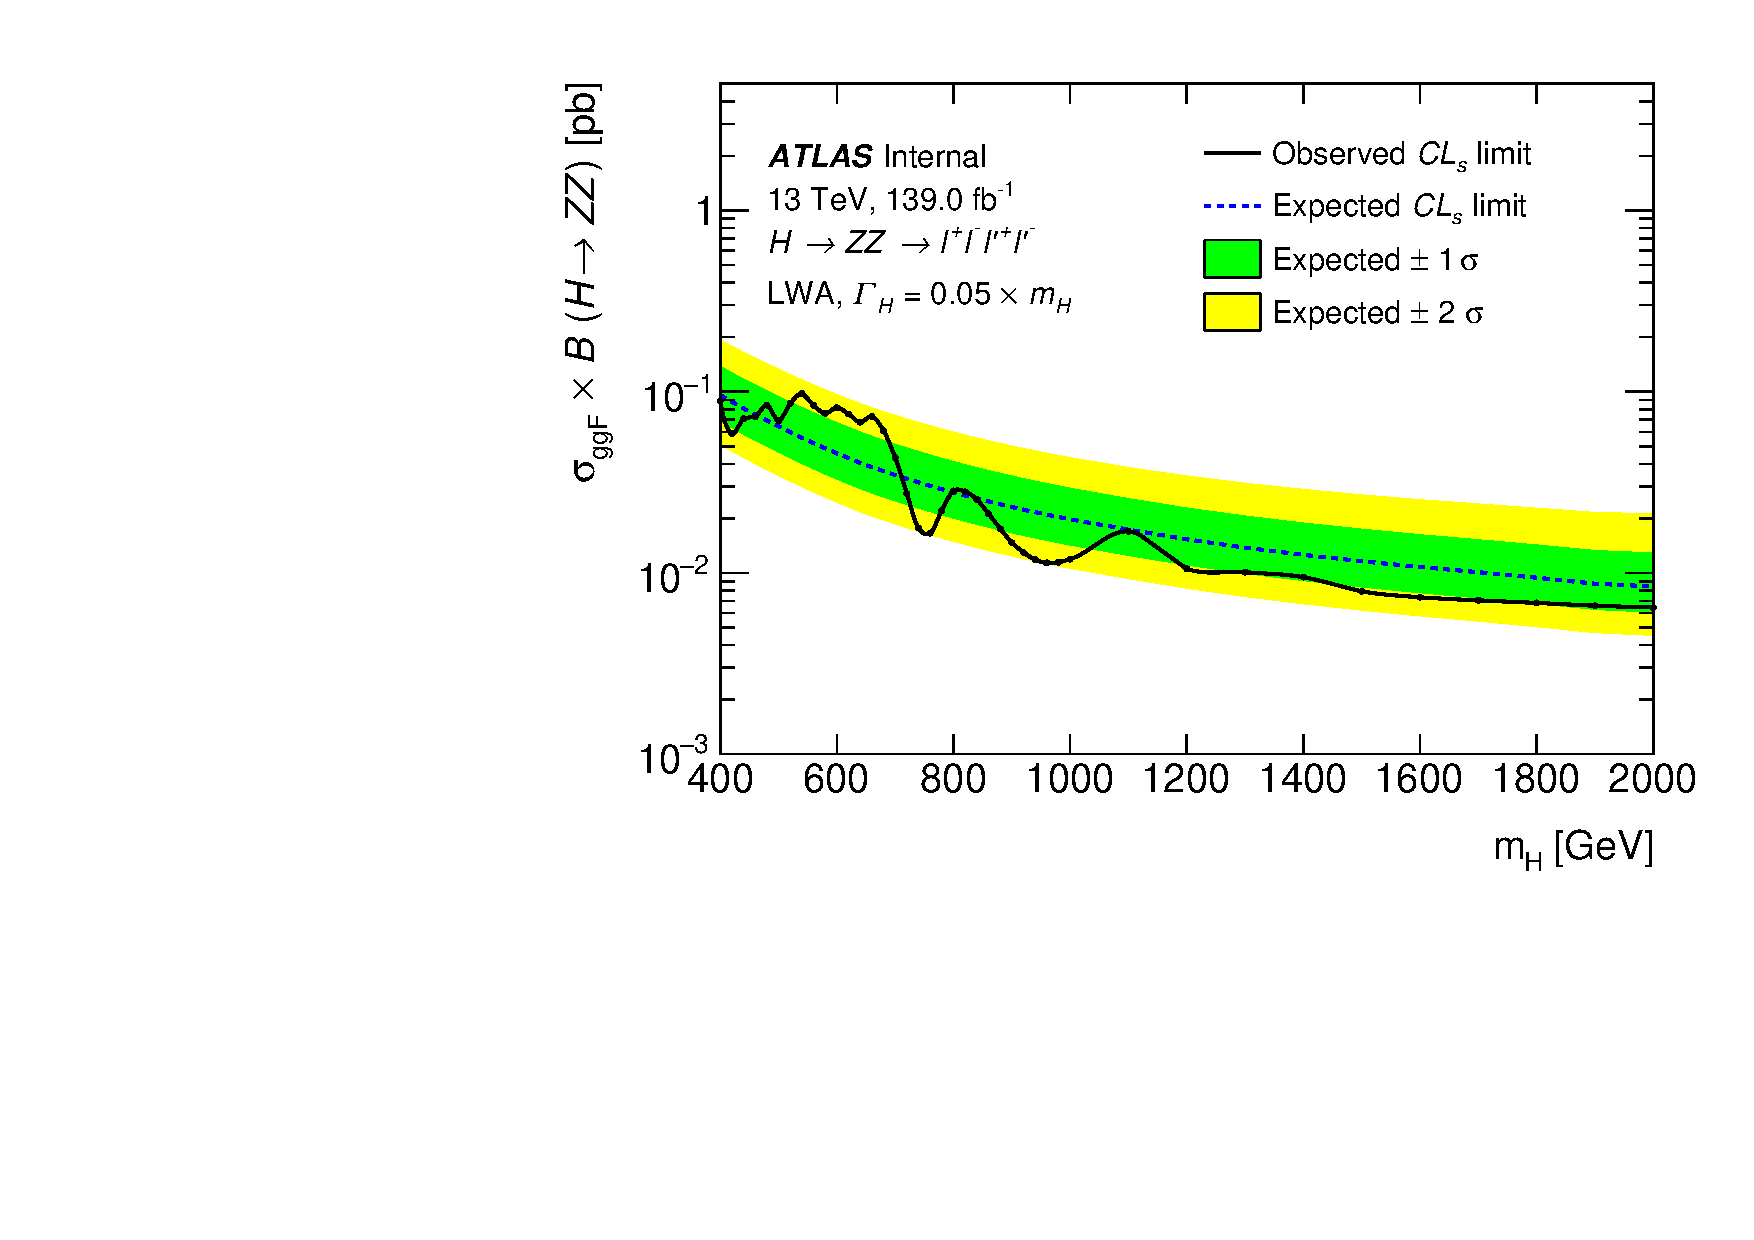
\includegraphics[width=0.48\textwidth]{figures/HMHZZ/results/Limits_LWA_withInt_5.pdf} \\
    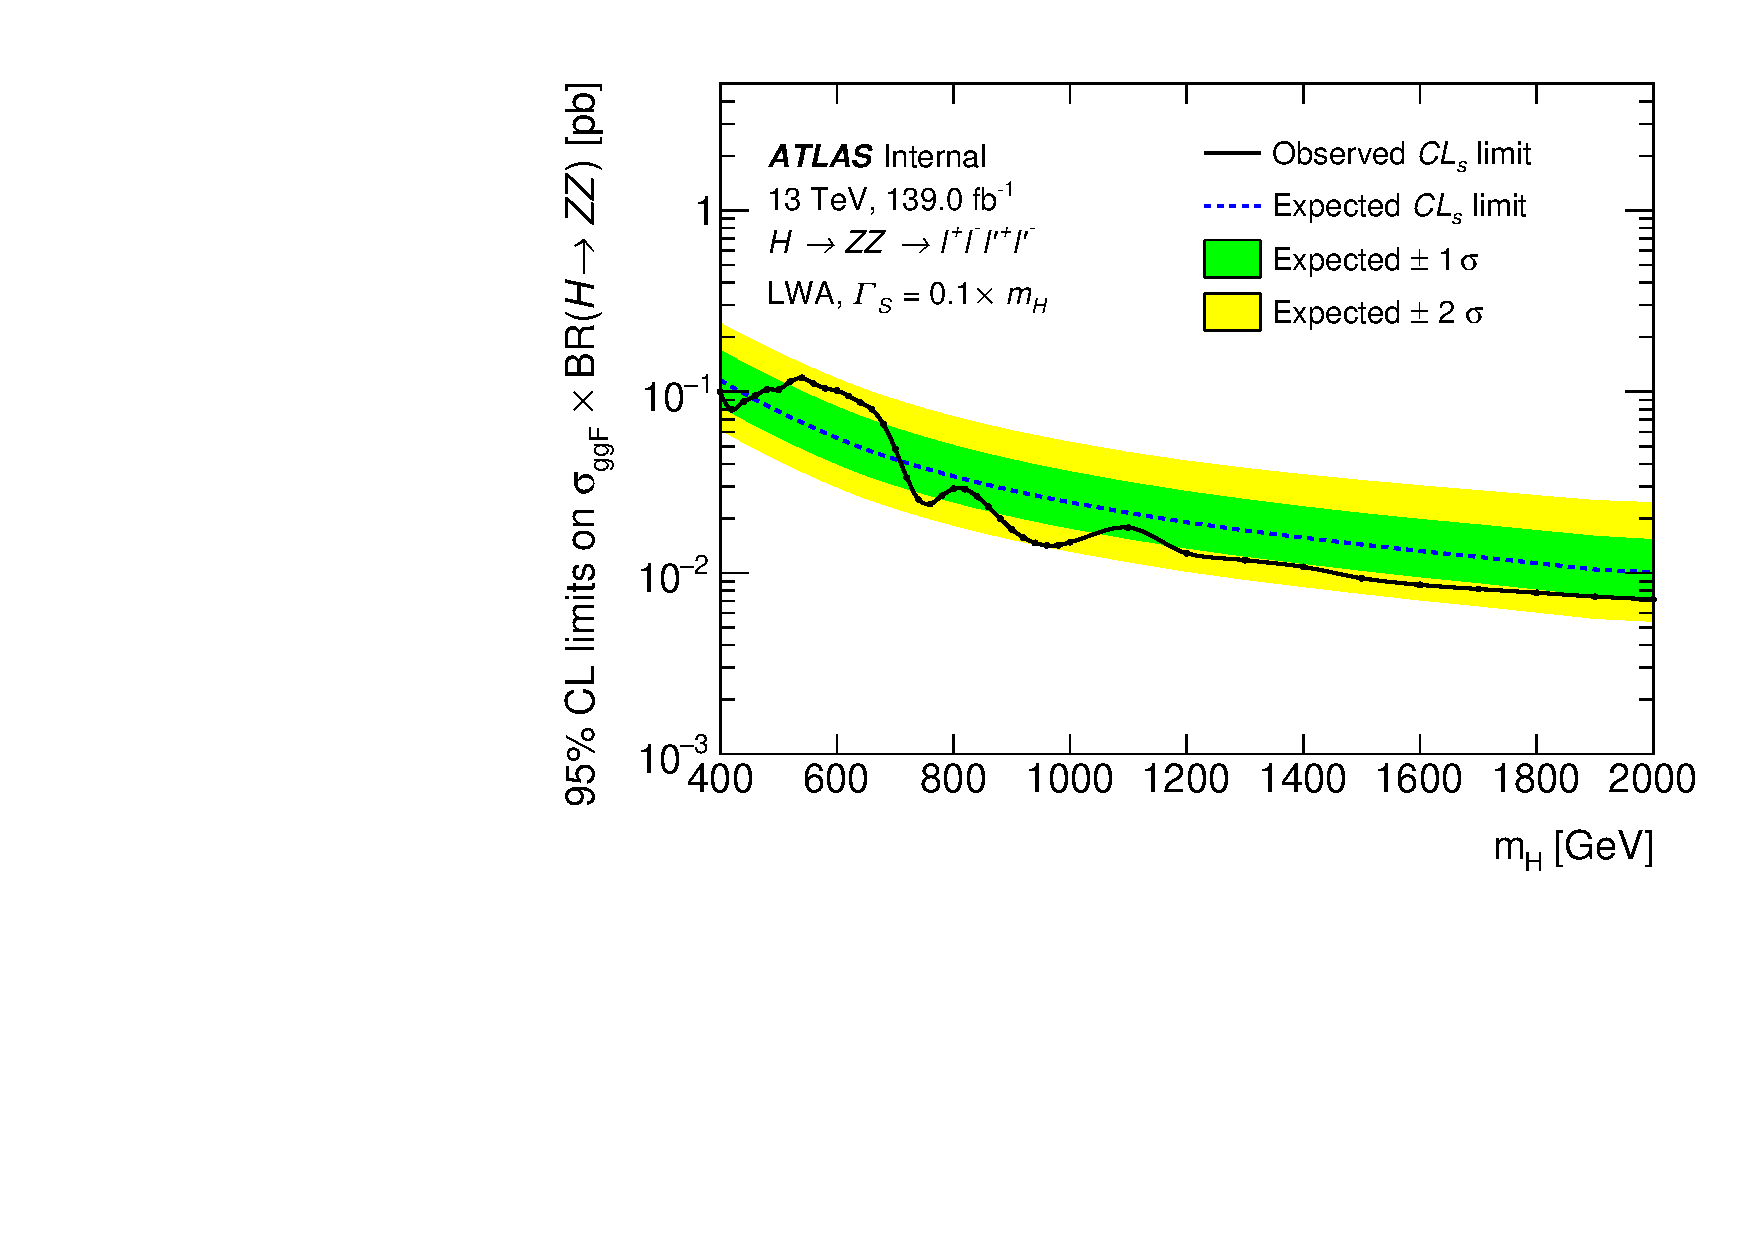
\includegraphics[width=0.48\textwidth]{figures/HMHZZ/results/Limits_LWA_withInt_10.pdf}
    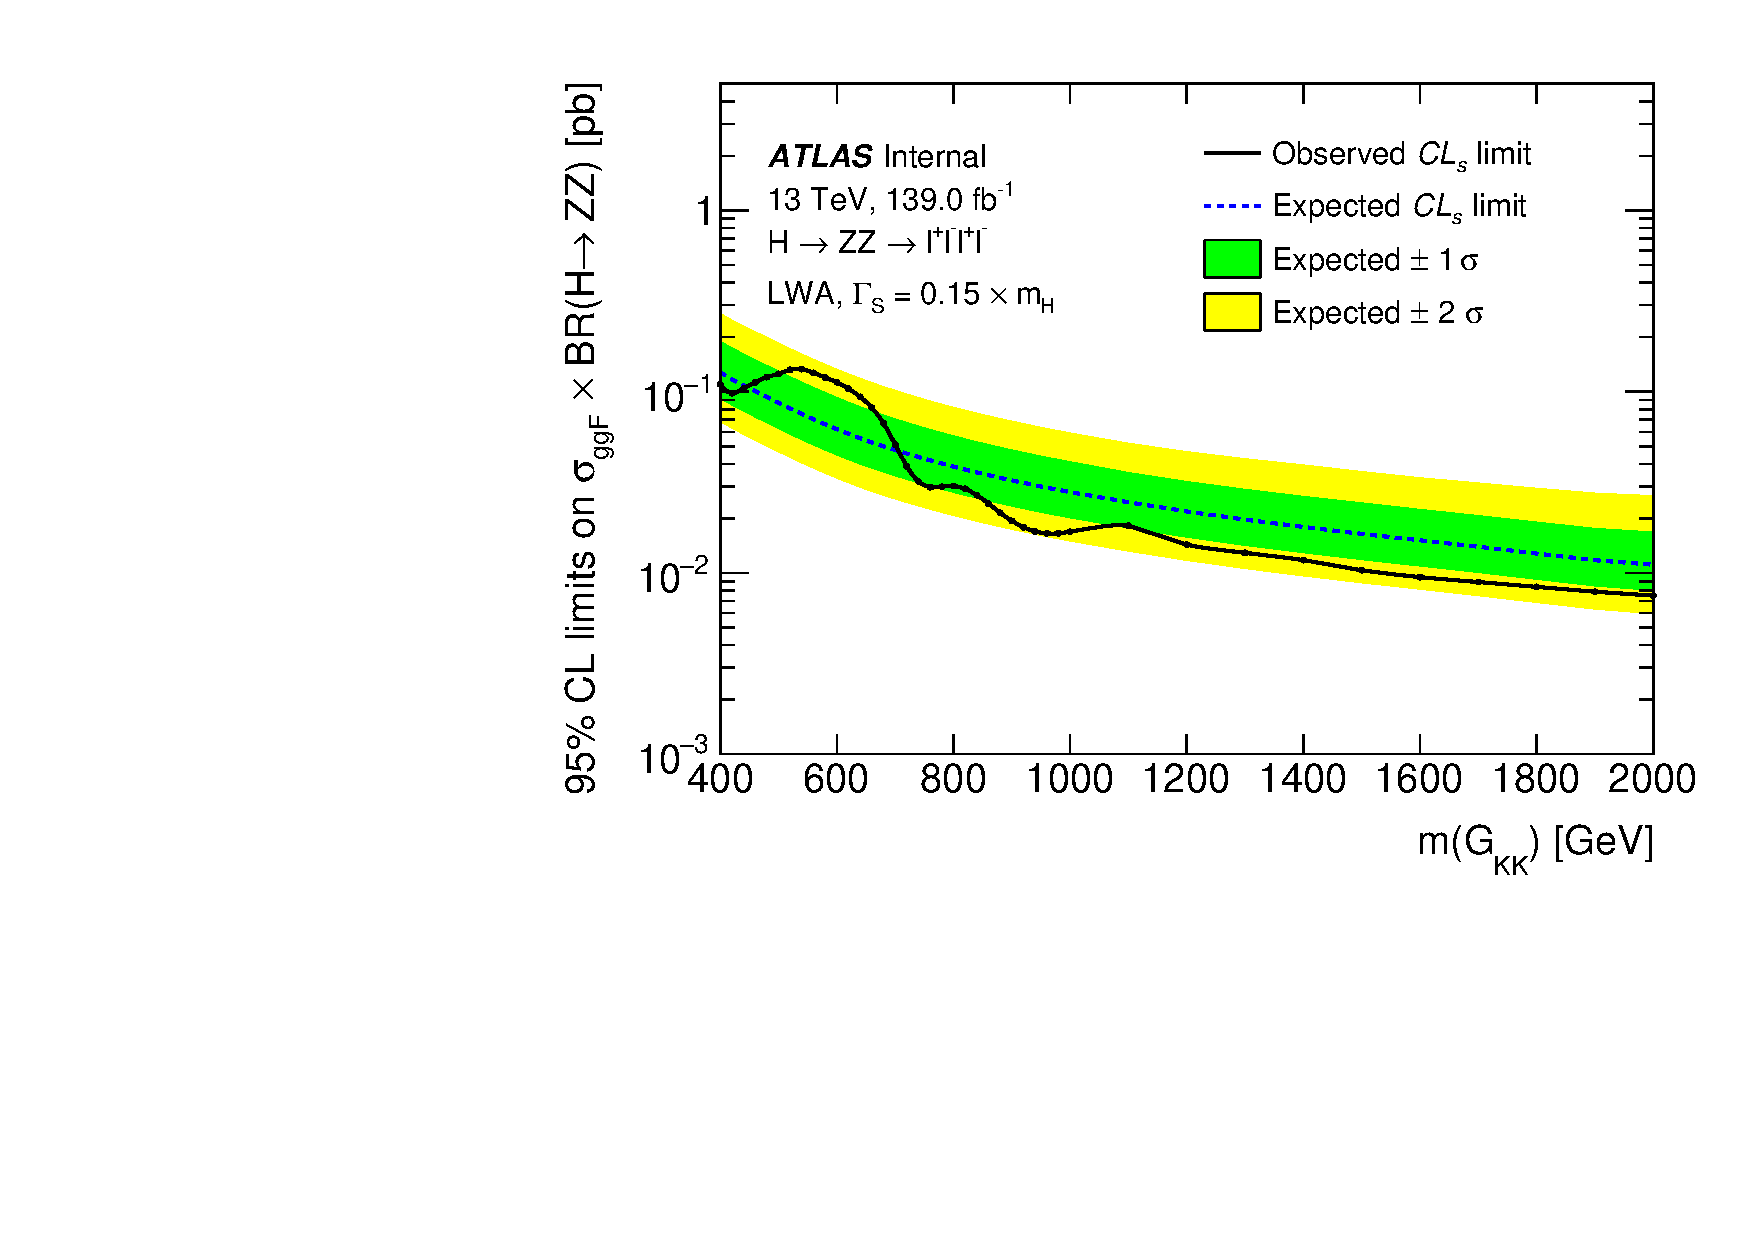
\includegraphics[width=0.48\textwidth]{figures/HMHZZ/results/Limits_LWA_withInt_15.pdf} \\
    \end{center}
    \caption{The upper limits at 95\% confidence level on $\sigma_{ggF} \times BR(H\rightarrow ZZ)$
    as a function of the heavy resonance mass $m_{H}$ for the ggF production mode with an intrinsic width of 1\% (top left), 5\% (top right), 10\% (bottom left) and 15\% (bottom right) for both the case where interference with Standard Model processes is considered.
    The green and yellow bands represent the $\pm 1~\sigma$ and $\pm 2~\sigma$ uncertainties in the expected limits.
  }
    \label{fig:LWAlimits_ggF_201518_withInt}
\end{figure}

\subsubsection{Spin-2 RS Graviton resonance}

The observed and expected 95\% upper limit on the cross section times branching ratio for RS Graviton (RSG) scenario is shown in figure~\ref{fig:RSGlimits_ggF_201518}.
Same as LWA case, only 4$e$, 4$\mu$ and 2$e$2$\mu$ channel of ggF production mode are used.
On top of the expected and observed upper limits in this model, a predicted cross section as function of mass provided by theorist is also shown in the figure.
Comparing with the observed result provided by $ZZ \rightarrow \llll$ decay, this spin-2 graviton is excluded up to a mass of 1500~\gev.

\begin{figure}[h]
    \begin{center}
    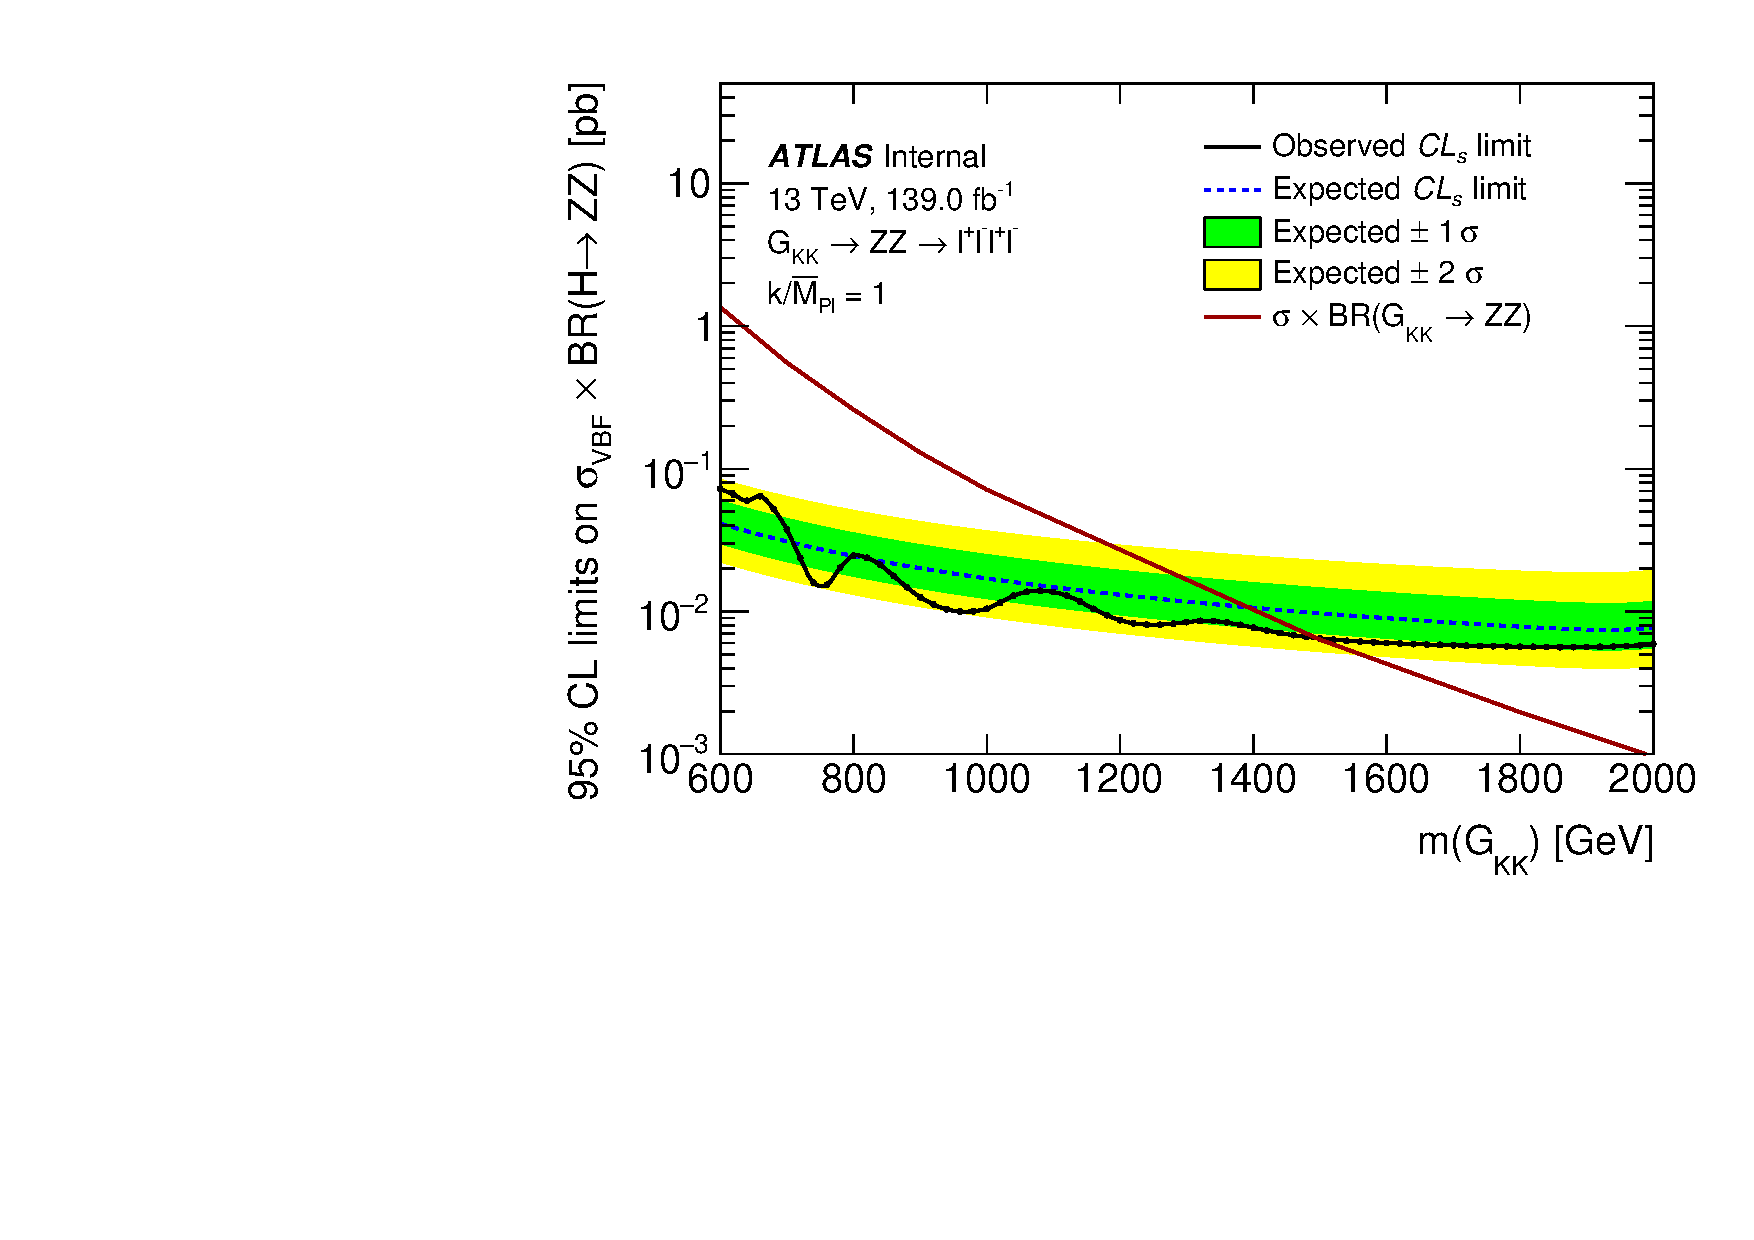
\includegraphics[width=0.48\textwidth]{figures/HMHZZ/results/Limits_RSG.pdf}
    \end{center}
    \caption{The upper limits at 95\% confidence level on $\sigma_{ggF} \times BR(G_{KK}\rightarrow ZZ)$
    as a function of the heavy resonance mass $m(G_{KK})$ for the ggF production mode in RS Graviton model.
    The green and yellow bands represent the $\pm 1~\sigma$ and $\pm 2~\sigma$ uncertainties in the expected limits.
  }
    \label{fig:RSGlimits_ggF_201518}
\end{figure}

\subsubsection{Summary of interpretation}

As a summary, figure~\ref{fig:models_limits} shows the comparison of expected and observed 95\% CL upper limits between different models described above.

\begin{figure}[h]
    \centering
    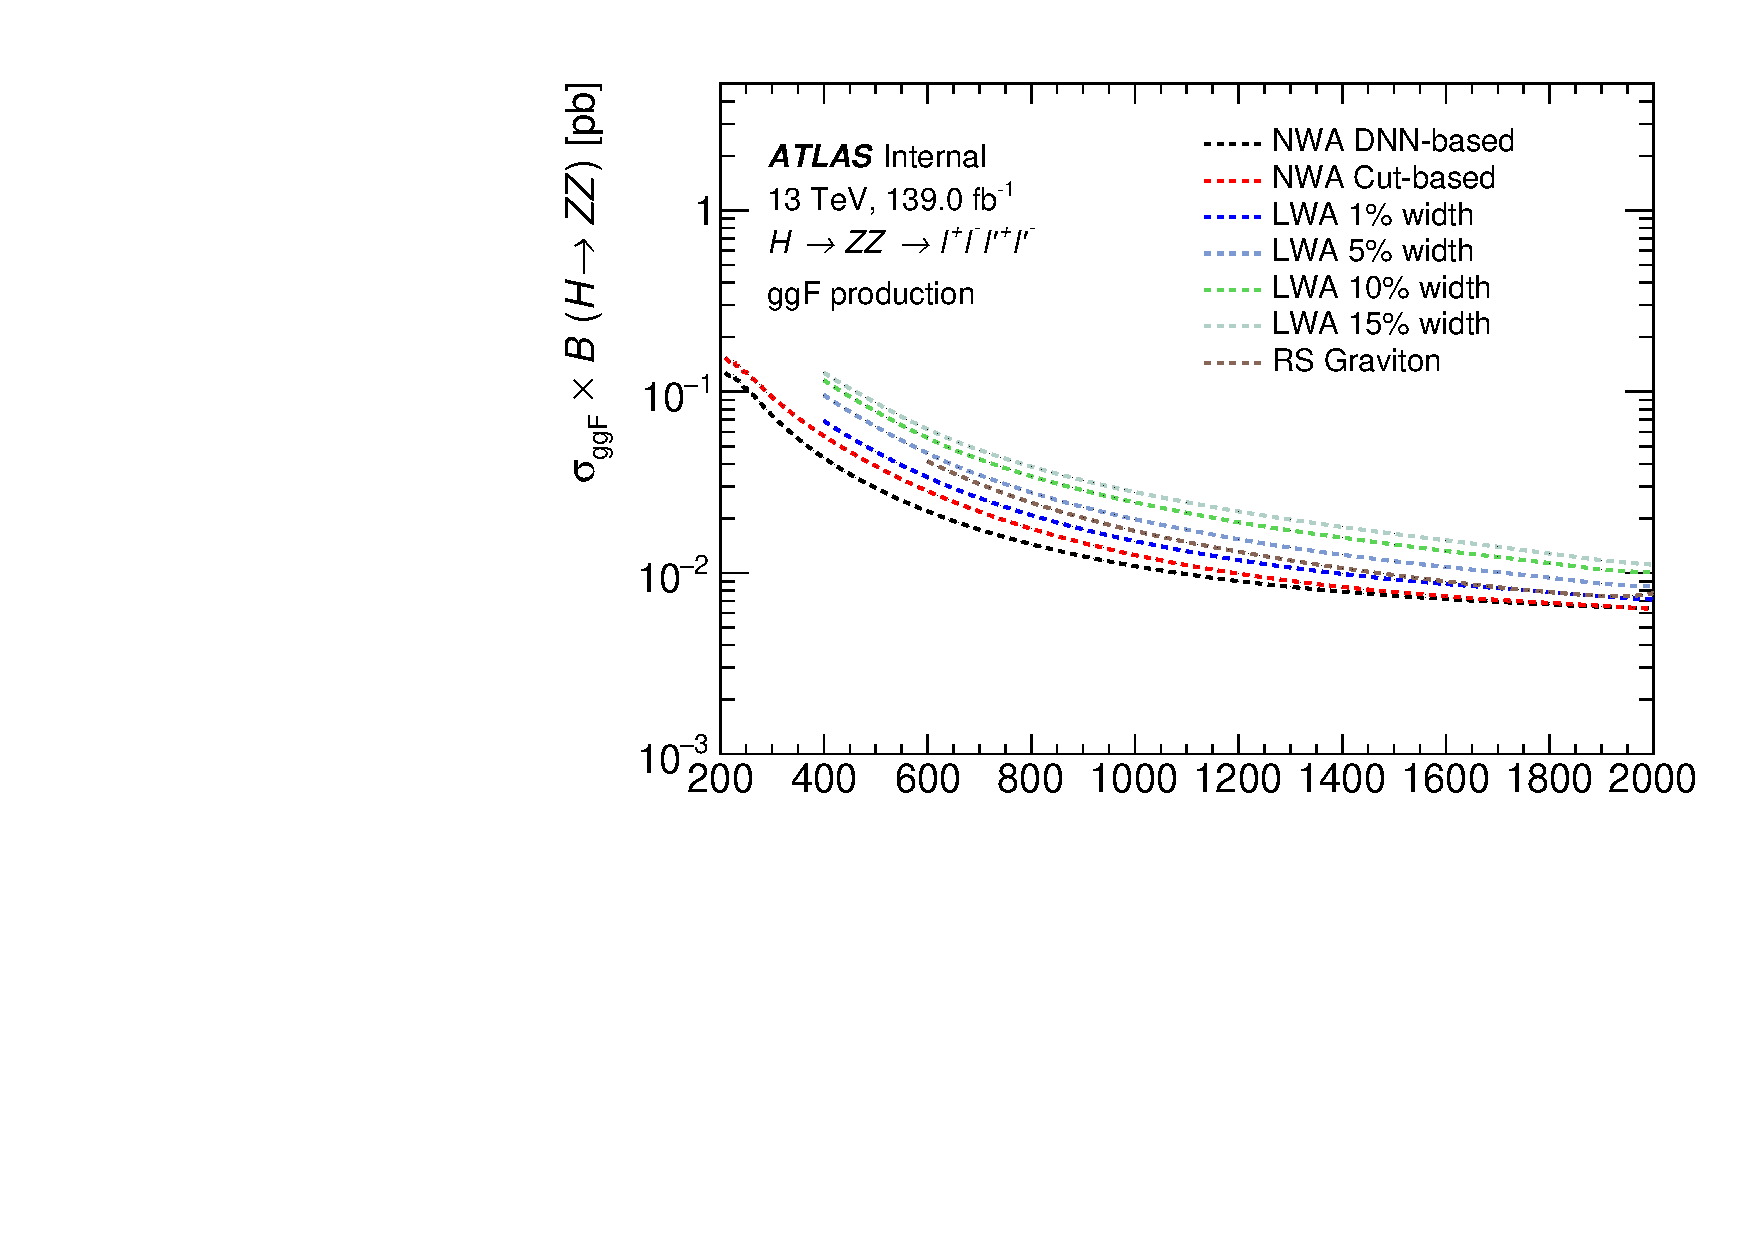
\includegraphics[width=0.48\textwidth]{figures/HMHZZ/results/4l_compareAll_exp.pdf}
    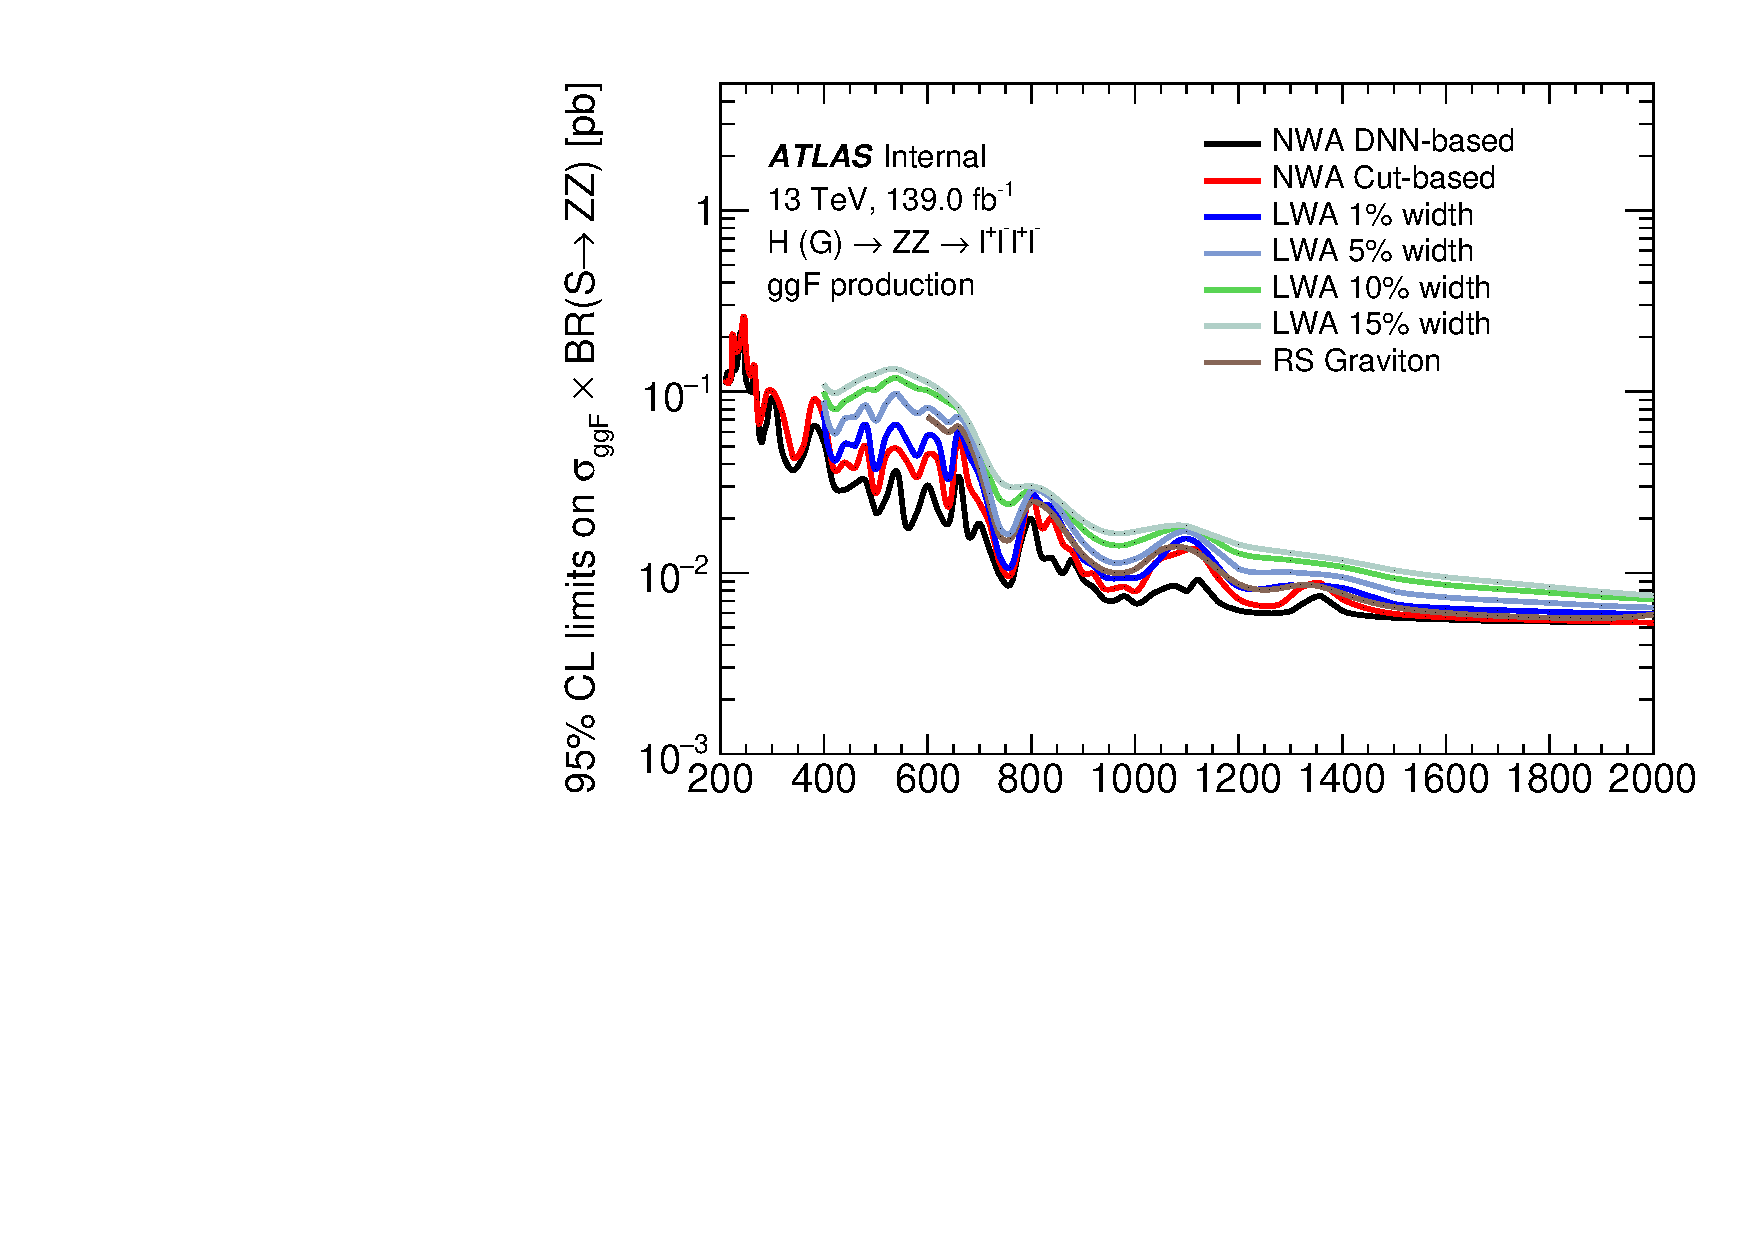
\includegraphics[width=0.48\textwidth]{figures/HMHZZ/results/4l_compareAll_obs.pdf}
    \caption{The expected (left) and observed (right) upper limits at 95\% confidence level on $\sigma \times BR(S\to ZZ)$ for ggF production mode at different assumptions. }
    \label{fig:models_limits}
\end{figure}

Figure~\ref{fig:comparison_limits} compares the expected 95\% CL upper limits as a function of the NWA resonance mass 
in this analysis with full run-2 data and the one in previous publication~\cite{Aaboud:2017rel} with the integrated luminosity of 36.1~\ifb.
With a significant increase of integrated luminosity and an improved analysis strategy, comparing to the previous publication,
the expected sensitivities of searching for narrow-width heavy resonance reduce by up to 70\% in MVA-based analysis,
where 50\% of reduction is due to luminosity increase while other improvement mainly comes from inviting multivariate method.

\begin{figure}[h]
    \centering
    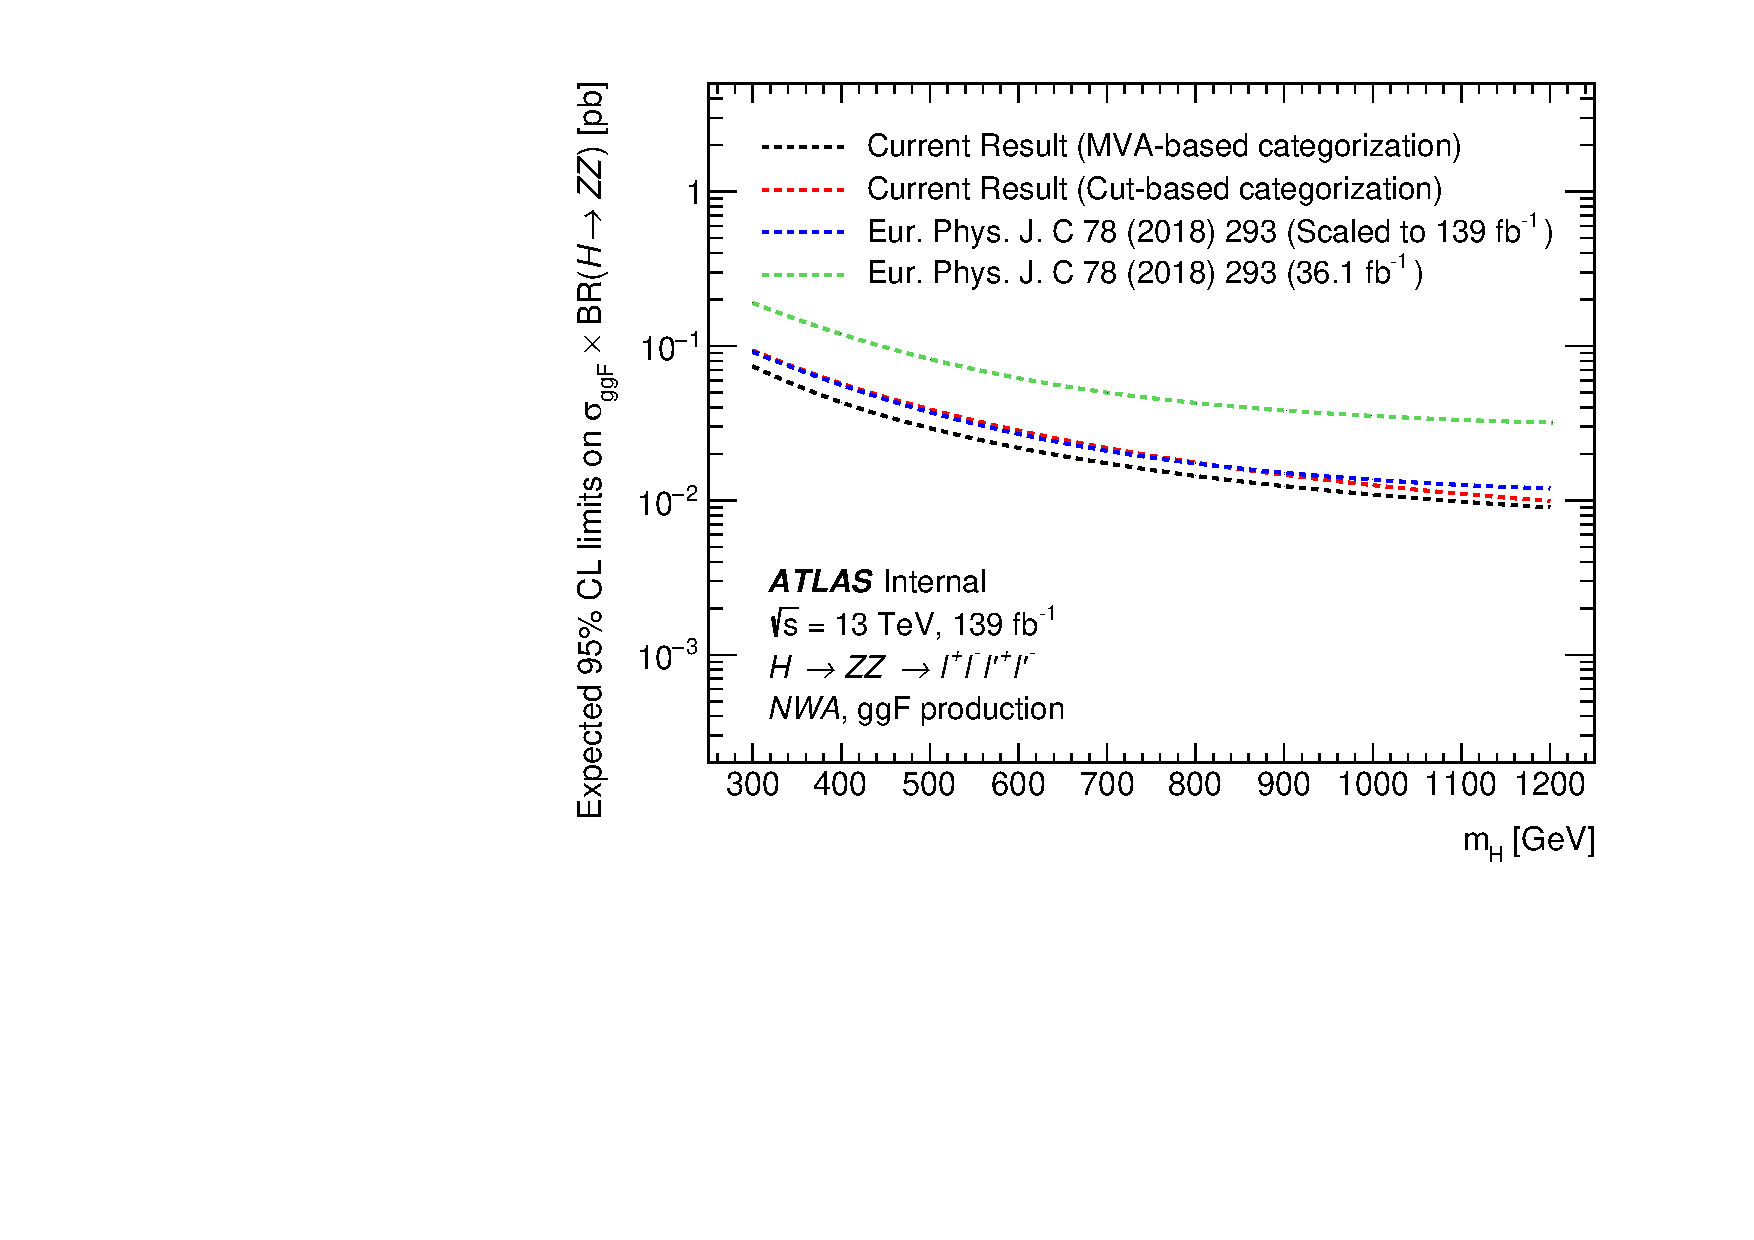
\includegraphics[width=0.48\textwidth]{figures/HMHZZ/results/4l_36vs139_ggF.pdf}
    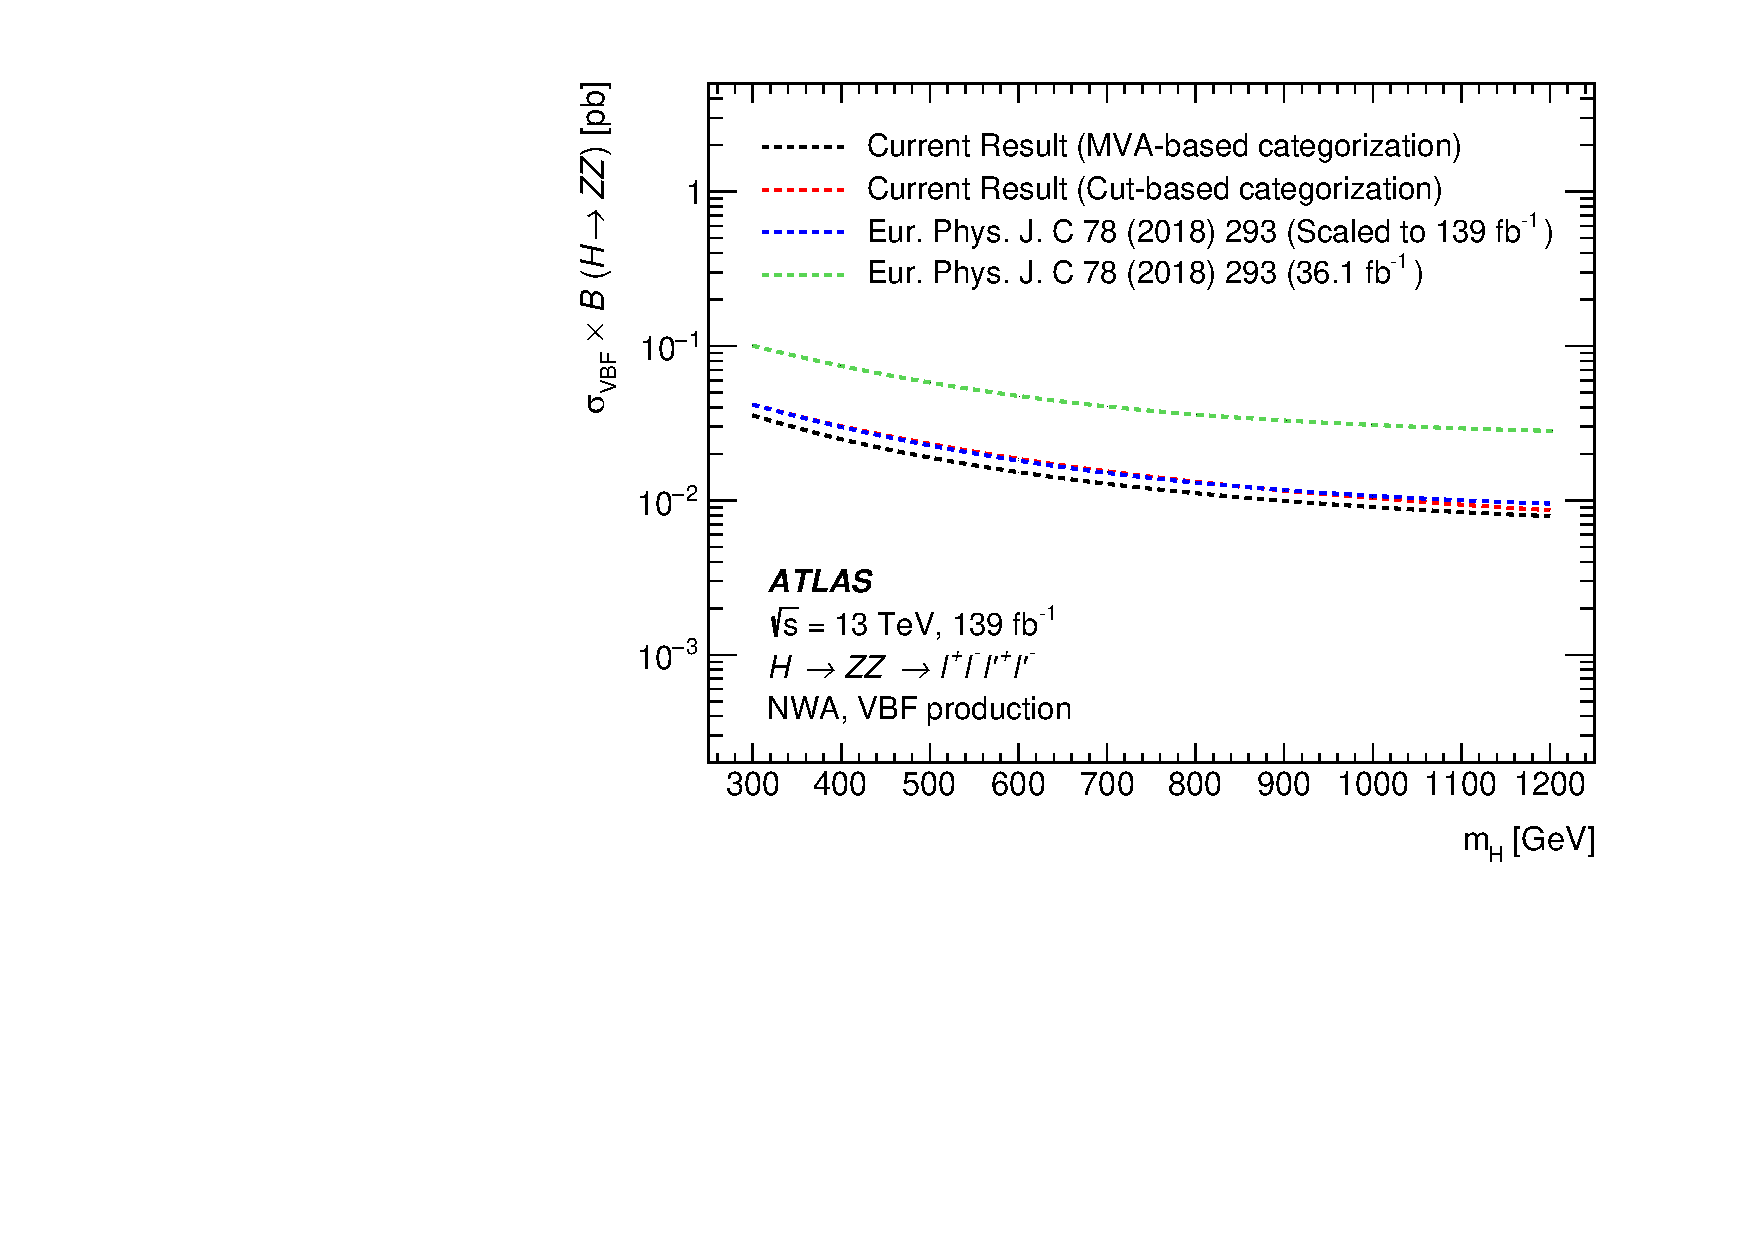
\includegraphics[width=0.48\textwidth]{figures/HMHZZ/results/4l_36vs139_VBF.pdf}
    \caption{Comparisons of the expected upper limits at 95\% CL on the cross section times branching ratio as a
             function of the heavy resonance mass ~\mH~ for the ggF production mode (left) and for the VBF production mode
             (right) in the case of the NWA. The expected limits from the previous publication are shown in the green dashed
             line and are projected to the 139~\ifb~
             as shown in the blue dashed line. In addition, the current results based on either
             cut-based categorisation or the multivariate-based categorisation are shown in red and black lines.}
    \label{fig:comparison_limits}
\end{figure}

Figure~\ref{fig:4mu_eventdisplay} shows the display of one candidate event passing analysis selection in four-muon final state with four-muon invariant mass of 1.34~\tev.

\begin{figure}[h]
    \centering
    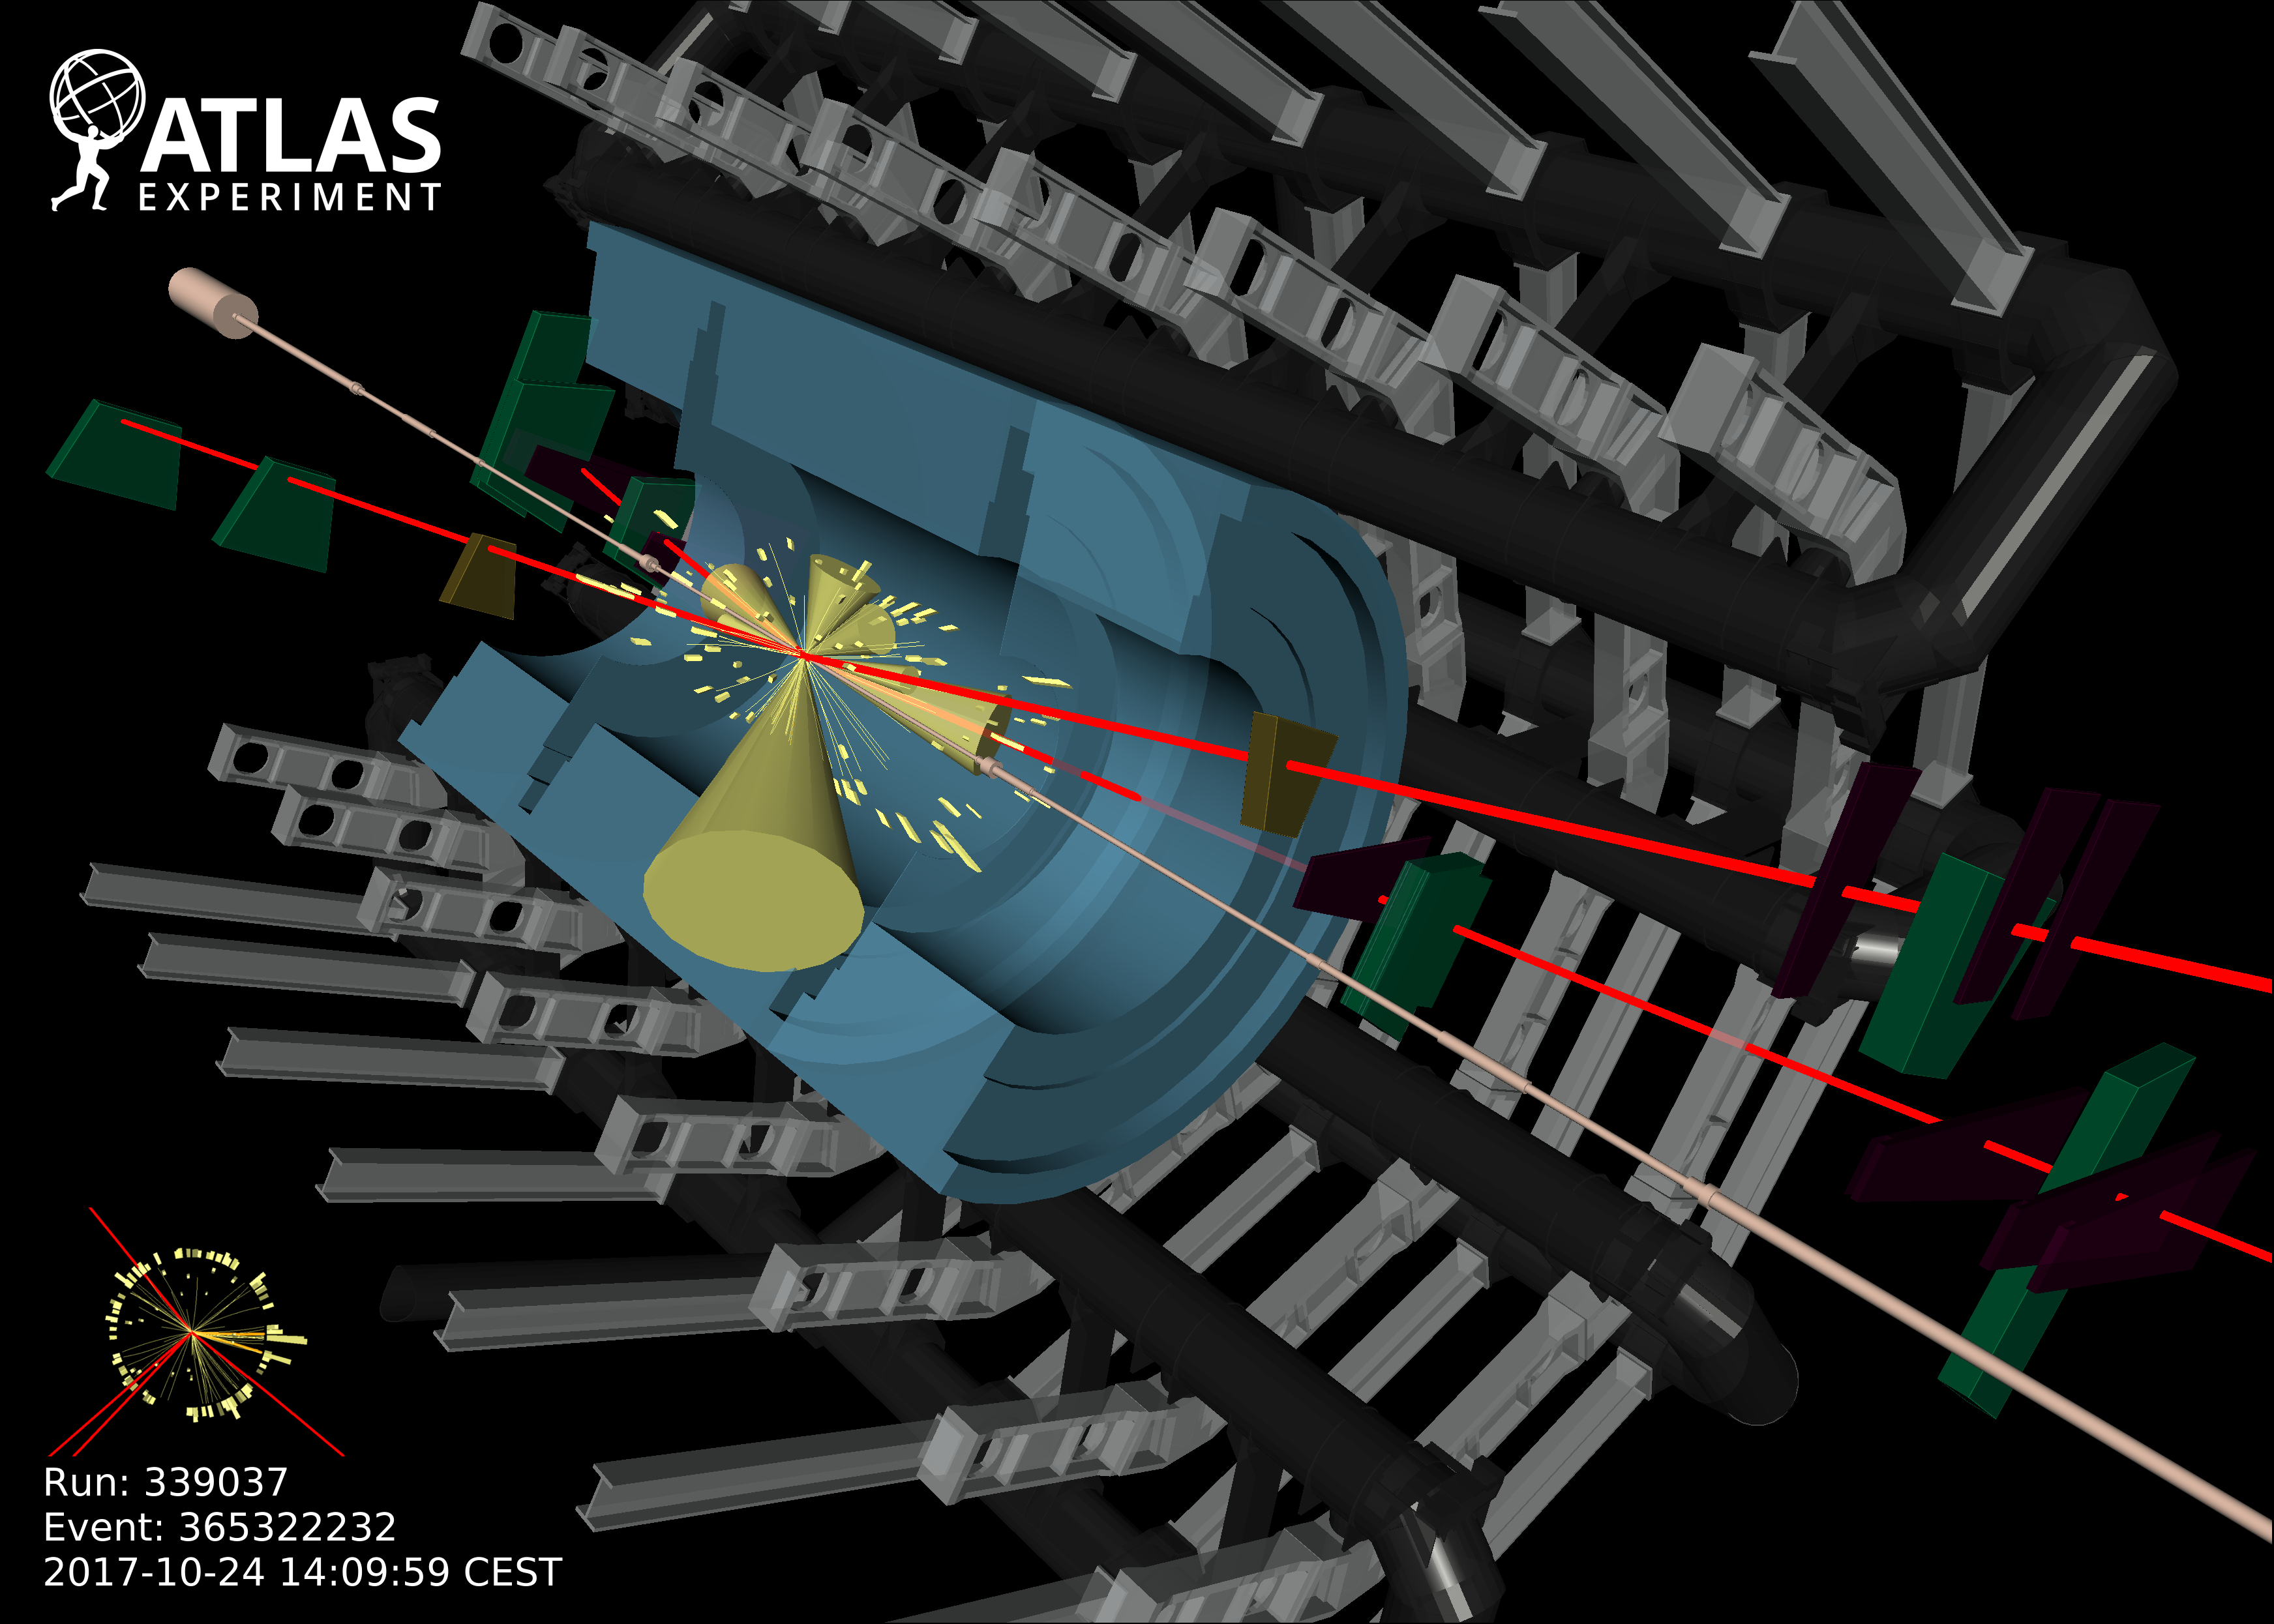
\includegraphics[width=1.0\textwidth]{figures/HMHZZ/results/display_run339037_evt365322232_2017-10-24T14-09-59.png}
    \caption{Display of one candidate event in 4$\mu$ final state with the mass of 1.35~\tev.}
    \label{fig:4mu_eventdisplay}
\end{figure}
